% ============================================================
% TESIS
% Reducción de imágenes CCD y fotometría instrumental
% Santiago Serrano Perico
% Universidad de los Andes
% ============================================================

\documentclass[12pt,letterpaper,oneside]{book}

\usepackage{astro-thesis}

% Paquetes adicionales
\usepackage{amsmath}
\usepackage{amssymb}
\usepackage{booktabs}
\usepackage{array}
\usepackage{graphicx}
\usepackage{float}
\usepackage{pdflscape}
\usepackage{multirow}
\usepackage{longtable}
\usepackage{url}
\usepackage{hyperref}

% ============================================================
% CONFIGURACIÓN GENERAL EN ESPAÑOL
% ============================================================

\addto\captionsspanish{
    \renewcommand{\contentsname}{Contenido}
    \renewcommand{\listfigurename}{Índice de figuras}
    \renewcommand{\listtablename}{Índice de tablas}
    \renewcommand{\bibname}{Bibliografía}
    \renewcommand{\appendixname}{Apéndice}
}


\begin{document}

% ============================================================
% PORTADA
% ============================================================

\begin{titlepage}

\begin{center}


\includegraphics[height=1.8cm]{img/logo-uniandes.pdf}

\vspace{2cm}

{\fontsize{23}{30}\selectfont
\bf
Desarrollo de un software para fotometría de apertura con selección adaptativa del anillo de
cielo
\par}


\vspace{18mm}

{\huge
Santiago Serrano Perico
}


\vspace{10mm}

{\large
Director:\\
Jose Alejandro Garcia Varela
}

\vspace{15mm}

{\Large
Facultad de Ciencias\\
Departamento de Física\\
Bogotá, Colombia\\
2026
}

\end{center}

\end{titlepage}


% ============================================================
% PÁGINAS PRELIMINARES
% ============================================================

\frontmatter


% ============================================================
% RESUMEN
% ============================================================

\chapter*{Resumen}

El análisis de imágenes astronómicas obtenidas con detectores CCD requiere una serie de procedimientos destinados a separar la señal producida por los objetos celestes de las contribuciones instrumentales y estadísticas introducidas durante la adquisición de los datos. En este trabajo se desarrolla e implementa un flujo de reducción y análisis fotométrico utilizando IRAF (\textit{Image Reduction and Analysis Facility}), aplicado principalmente a imágenes de los cúmulos estelares M92 y M41.

El trabajo comprende tres etapas principales. En la primera se realiza la reducción de imágenes CCD del cúmulo globular M92 mediante procedimientos de inspección de encabezados FITS, corrección por \textit{overscan}, recorte de la región útil del detector, corrección por \textit{bias} y corrección por \textit{flat field}. En la segunda etapa se estudia la identificación y caracterización manual de fuentes estelares mediante las herramientas \texttt{display} e \texttt{imexamine} de IRAF, con especial atención a la determinación del ancho a media altura, FWHM (\textit{Full Width at Half Maximum}), y a la caracterización estadística del fondo de cielo.

En la tercera etapa se realiza fotometría de apertura sobre imágenes de M92 y M41. Para ello se estudian parámetros como el radio de apertura, el FWHM, el nivel de ruido del cielo y el umbral de detección utilizado por \texttt{daofind}. Se adopta una apertura correspondiente a tres veces la mediana del FWHM de cada imagen y un umbral de detección (\texttt{threshold}) de 3.5. Posteriormente se obtienen magnitudes instrumentales y errores fotométricos mediante \texttt{phot} y \texttt{qphot}.

Para M92 se construye además un diagrama color--magnitud instrumental utilizando observaciones en los filtros $B$ y $V$. Como parte del proceso de depuración de la muestra fotométrica se implementan dos criterios adicionales. El primero utiliza el algoritmo de vecinos más cercanos para eliminar fuentes que poseen otra estrella dentro de una distancia de $3\times FWHM$. El segundo analiza la distribución de cuentas en los anillos utilizados para determinar el fondo local, identificando posibles casos de contaminación por fuentes vecinas.

Los resultados permiten establecer un procedimiento reproducible para pasar desde una imagen CCD cruda hasta una muestra de fuentes adecuada para análisis fotométrico. El trabajo muestra además la importancia de la reducción instrumental, la selección de parámetros fotométricos y la inspección de fuentes contaminadas en campos estelares relativamente densos.

\vspace{5mm}

\noindent
\textbf{Palabras clave:}
CCD, fotometría de apertura, IRAF, M92, M41, FWHM, diagrama color--magnitud, reducción de imágenes.


% ============================================================
% RESUMEN EN INGLÉS
% ============================================================

\chapter*{Resumen en inglés}

Astronomical images obtained with CCD detectors require several processing stages to separate the signal produced by astronomical sources from instrumental and statistical contributions introduced during data acquisition. This work develops and implements a CCD reduction and aperture-photometry workflow using IRAF (\textit{Image Reduction and Analysis Facility}), mainly applied to observations of the stellar clusters M92 and M41.

The procedure includes CCD image reduction, manual and automatic stellar-source identification, estimation of the stellar FWHM and local sky background, automatic source detection, aperture photometry, instrumental magnitude determination, and construction of an instrumental color--magnitude diagram for M92.

An aperture radius corresponding to three times the median stellar FWHM was adopted, while a detection threshold of 3.5 times the background noise was used for automatic source detection. Additional quality criteria based on nearest-neighbor distances and possible contamination of the sky annulus were implemented to improve the final photometric sample.

The resulting workflow provides a practical framework for processing CCD observations and obtaining instrumental photometric measurements suitable for subsequent photometric calibration and stellar-population analysis.

\vspace{5mm}

\noindent
\textbf{Palabras clave en inglés:}
CCD, aperture photometry, IRAF, M92, M41, FWHM, color--magnitude diagram.


% ============================================================
% CONTENIDO
% ============================================================

\mainmatter

\tableofcontents

\newpage

\listoffigures

\listoftables


\newpage

\visibleintentfalse


% ============================================================
% CAPÍTULO 1
% INTRODUCCIÓN
% ============================================================

\chapter{Introducción}

La astronomía observacional depende de la capacidad de transformar la radiación proveniente de objetos celestes en mediciones cuantitativas. Durante gran parte de la historia de la astronomía estas observaciones se realizaron visualmente o mediante placas fotográficas. Sin embargo, el desarrollo de los dispositivos de carga acoplada, conocidos como CCD por sus siglas en inglés \textit{Charge-Coupled Device}, transformó profundamente la adquisición de datos astronómicos.

Los CCD presentan ventajas importantes para la astronomía, entre ellas una alta eficiencia cuántica, una respuesta aproximadamente lineal dentro de un intervalo amplio de señal, buena estabilidad y la posibilidad de representar digitalmente la intensidad de la radiación incidente en cada elemento del detector. Estas características permiten realizar mediciones fotométricas con una precisión considerablemente superior a muchos detectores utilizados históricamente.

Una imagen astronómica CCD no debe entenderse solamente como una representación visual del cielo. Cada imagen consiste en una matriz bidimensional de valores numéricos en la que cada píxel contiene información relacionada con la cantidad de carga producida durante la exposición. Esta carga está asociada principalmente a los fotones provenientes del objeto astronómico y del fondo de cielo, pero también contiene contribuciones electrónicas producidas por el propio detector y por su sistema de lectura.

Por esta razón, las imágenes obtenidas directamente durante una observación no suelen estar inmediatamente preparadas para realizar mediciones científicas. Antes de extraer posiciones, flujos o magnitudes es necesario aplicar un proceso de reducción destinado a corregir efectos instrumentales como el nivel de \textit{bias}, las variaciones observadas mediante el \textit{overscan}, la corriente oscura y las diferencias en sensibilidad entre diferentes regiones del detector.

Una vez realizada la reducción, las imágenes pueden utilizarse para medir el brillo de los objetos astronómicos. El procedimiento mediante el cual se mide la cantidad de radiación proveniente de un objeto se denomina fotometría.

En el caso de estrellas observadas mediante imágenes CCD, uno de los métodos más utilizados es la fotometría de apertura. El procedimiento consiste en integrar las cuentas dentro de una región circular centrada sobre la estrella y posteriormente estimar y restar la contribución local del fondo de cielo.

Sin embargo, la precisión del resultado depende de diferentes parámetros. Entre ellos se encuentran el tamaño de la apertura, la estimación del fondo local, el FWHM de las fuentes, la relación señal--ruido, la presencia de estrellas cercanas y la posibilidad de contaminación dentro de la apertura o dentro del anillo utilizado para calcular el cielo.

El software IRAF proporciona herramientas para realizar cada una de estas etapas. Mediante tareas especializadas es posible inspeccionar imágenes FITS, realizar reducción CCD, medir perfiles estelares, detectar fuentes automáticamente, efectuar fotometría y extraer los resultados para análisis posterior.

En este trabajo se implementa un flujo de reducción y fotometría utilizando IRAF, aplicado a imágenes de los cúmulos M92 y M41. El procedimiento se desarrolló inicialmente a través de tres talleres: reducción CCD, identificación manual de fuentes y fotometría de apertura. Posteriormente, el análisis se extendió mediante la construcción de un diagrama color--magnitud para M92 y mediante criterios adicionales destinados a seleccionar fuentes fotométricamente más confiables.

Los cúmulos estelares son particularmente apropiados para este tipo de análisis porque contienen numerosas estrellas observadas aproximadamente a una misma distancia y, en primera aproximación, asociadas a una misma población. Un diagrama color--magnitud permite ordenar dichas estrellas de acuerdo con su luminosidad y su color, proporcionando información fundamental sobre las características de la población estelar.

Este trabajo constituye por tanto una introducción práctica y teórica al procesamiento de imágenes CCD y a la fotometría estelar, y establece las bases para una futura calibración fotométrica y un análisis más detallado de las propiedades físicas de M92.


% ============================================================
% MARCO TEÓRICO INTEGRADO EN LA INTRODUCCIÓN
% ============================================================

\section{Marco teórico}


% ============================================================
% CCD
% ============================================================

\subsection{Detectores CCD}

Los dispositivos de carga acoplada o CCD son detectores de estado sólido capaces de convertir fotones incidentes en carga eléctrica. Su utilización revolucionó la astronomía observacional debido a su sensibilidad, estabilidad y capacidad para realizar mediciones cuantitativas de la radiación incidente.

De acuerdo con Howell \cite{howell2006}, una de las principales ventajas de un CCD es que la información se registra directamente en una matriz digital. Cada elemento de esta matriz corresponde a un píxel físico del detector.

Cuando un fotón posee energía suficiente y es absorbido por el material semiconductor del CCD, puede liberar un electrón. Durante el tiempo de exposición, los electrones producidos se acumulan dentro de los correspondientes pozos de potencial asociados a cada píxel.

Al finalizar la exposición, las cargas almacenadas se transfieren secuencialmente hacia la electrónica de salida del detector. Allí se convierten primero en una señal de voltaje y posteriormente en un valor digital.

El número registrado en la imagen no necesariamente corresponde directamente al número de electrones generados. Habitualmente la señal digital se almacena en unidades denominadas ADU, \textit{Analog-to-Digital Units}.


% ------------------------------------------------------------
\subsection{Eficiencia cuántica}

La eficiencia cuántica, generalmente representada por $QE$, describe la fracción de fotones incidentes que producen electrones detectables.

Puede expresarse de manera simplificada como

\[
QE =
\frac{N_{e^-}}{N_{\gamma}},
\]

donde $N_{e^-}$ corresponde al número de electrones generados y $N_{\gamma}$ al número de fotones incidentes.

Una eficiencia cuántica mayor implica que una fracción más grande de los fotones recibidos contribuye a la señal medida.

La eficiencia cuántica generalmente depende de la longitud de onda. Por esta razón, la respuesta de un CCD no es necesariamente idéntica en todo el espectro electromagnético.


% ------------------------------------------------------------
\subsection{Ganancia del detector}

La electrónica de lectura transforma el número de electrones acumulados en un valor digital. La relación entre electrones y ADU se describe mediante la ganancia del detector.

Si $g$ representa la ganancia en unidades de electrones por ADU, entonces

\[
N_{e^-} = g\,N_{\rm ADU}.
\]

El conocimiento de la ganancia es particularmente importante cuando se realiza un cálculo cuantitativo de la relación señal--ruido, ya que el ruido de Poisson se encuentra naturalmente expresado en electrones.


% ------------------------------------------------------------
\subsection{Linealidad y saturación}

Dentro de su región de funcionamiento normal, un CCD ideal presenta una respuesta aproximadamente lineal: un incremento proporcional en el número de fotones incidentes produce un incremento proporcional en la señal medida.

Esta propiedad es fundamental para la fotometría.

Sin embargo, cada píxel posee una capacidad máxima de almacenamiento de carga. Cuando la señal supera este límite, el píxel alcanza la saturación y deja de responder linealmente al flujo incidente.

Las estrellas saturadas no son apropiadas para fotometría convencional, ya que sus cuentas dejan de representar correctamente su flujo real.


% ============================================================
% IMAGEN CCD
% ============================================================

\subsection{Componentes de una imagen CCD}

Una imagen CCD cruda contiene diferentes contribuciones.

De forma conceptual puede representarse como

\[
I_{\rm raw}
=
I_{\star}
+
I_{\rm sky}
+
I_{\rm bias}
+
I_{\rm dark}
+
N,
\]

donde

En esta expresión, $I_{\star}$ representa la señal producida por los objetos astronómicos, $I_{\rm sky}$ corresponde a la contribución del fondo de cielo, $I_{\rm bias}$ al nivel electrónico de lectura, $I_{\rm dark}$ a la señal térmica y $N$ agrupa las diferentes contribuciones estadísticas de ruido.

Adicionalmente, la respuesta de cada píxel puede diferir ligeramente de la de otros píxeles. Esta variación se corrige mediante imágenes de \textit{flat field}.


% ============================================================
% BIAS
% ============================================================

\subsection{Nivel de polarización (\textit{bias})}

El \textit{bias} es un nivel electrónico añadido deliberadamente durante el proceso de lectura del CCD.

El sistema evita de esta manera que pequeñas fluctuaciones electrónicas produzcan valores digitales negativos.

Como consecuencia, incluso una exposición de tiempo prácticamente cero tomada con el obturador cerrado presenta una señal diferente de cero.

Una imagen de \textit{bias} permite medir esta contribución electrónica.

Idealmente se toman múltiples imágenes de \textit{bias}. Estas pueden combinarse para producir un \textit{master bias} con menor ruido estadístico.

Si $B_i(x,y)$ representa cada una de las imágenes de bias, el master puede calcularse mediante una media o mediana de las exposiciones:

\[
B_{\rm master}(x,y)
=
{\rm median}
\left[
B_1(x,y),
B_2(x,y),
\ldots,
B_n(x,y)
\right].
\]

El uso de la mediana posee la ventaja de reducir la influencia de valores atípicos.


% ============================================================
% OVERSCAN
% ============================================================

\subsection{Región de sobrelectura (\textit{overscan})}

La región de \textit{overscan} está formada por columnas o filas adicionales que son leídas por la electrónica del detector pero que no corresponden a píxeles físicamente expuestos a la luz.

Por esta razón, su nivel está asociado principalmente a la electrónica de lectura.

El \textit{overscan} permite estimar el nivel de \textit{bias} presente específicamente durante cada exposición.

Esta distinción es importante porque el nivel electrónico puede presentar pequeñas variaciones temporales.

Mientras que un \textit{master bias} caracteriza una estructura promedio del detector, el \textit{overscan} permite determinar posibles cambios en el nivel base de una imagen individual.

En IRAF la región correspondiente al overscan puede definirse mediante el parámetro

\begin{verbatim}
biassec
\end{verbatim}

de la tarea \texttt{ccdproc}.


% ============================================================
% TRIM
% ============================================================

\subsection{Recorte de la imagen}

Después de utilizar la región de \textit{overscan}, esta zona deja de ser necesaria para el análisis científico.

El procedimiento denominado \textit{trim} consiste en conservar únicamente la región útil del detector.

Además del overscan, el recorte puede eliminar bordes o regiones que no contienen información científica confiable.

En IRAF la región útil se define mediante \texttt{trimsec}.

En el proceso desarrollado durante este trabajo se utilizó una región de la forma

\begin{verbatim}
trimsec = [1:315,2:510]
\end{verbatim}

cuando correspondió a la configuración particular de las imágenes procesadas.


% ============================================================
% DARK
% ============================================================

\subsection{Corriente oscura}

Incluso en ausencia de radiación incidente, la energía térmica del detector puede generar electrones.

Este fenómeno recibe el nombre de corriente oscura o \textit{dark current}.

En términos generales, la señal de corriente oscura aumenta con el tiempo de exposición y depende fuertemente de la temperatura del detector.

La refrigeración del CCD permite reducir considerablemente esta contribución.

Cuando es necesario realizar una corrección de corriente oscura se adquieren exposiciones con el obturador cerrado y tiempos de integración conocidos.

Después de corregirlas por bias, las imágenes pueden combinarse para producir un \textit{master dark}.


% ============================================================
% FLAT
% ============================================================

\subsection{Corrección de campo plano (\textit{flat field})}

Incluso cuando una superficie uniformemente iluminada es observada por un CCD, los valores registrados no son perfectamente uniformes.

Existen diferencias de sensibilidad entre píxeles, además de efectos producidos por la óptica como viñeteo, sombras de partículas de polvo y gradientes de iluminación.

Estas variaciones se corrigen mediante imágenes conocidas como \textit{flat fields}.

El procedimiento consiste en observar una fuente aproximadamente uniforme. Posteriormente, la imagen de flat se corrige por los efectos electrónicos correspondientes y se normaliza.

Si $F(x,y)$ es un flat corregido, puede normalizarse como

\[
F_{\rm norm}(x,y)
=
\frac{F(x,y)}
{\langle F(x,y)\rangle}.
\]

La imagen científica corregida puede entonces expresarse aproximadamente como

\begin{equation}
I_{\rm corr}(x,y)
=
\frac{
I_{\rm raw}(x,y)
-
B(x,y)
-
D(x,y)
}
{
F_{\rm norm}(x,y)
}.
\end{equation}

Esta expresión representa de manera conceptual el proceso general. El procedimiento específico depende de la estructura de los datos y del detector utilizado.


% ============================================================
% RUIDO
% ============================================================

\subsection{Fuentes de ruido en imágenes CCD}

Las mediciones realizadas con un CCD contienen incertidumbre. Algunas de las fuentes más importantes son:

Las principales contribuciones a la incertidumbre son el ruido de Poisson asociado a los fotones de la estrella y del fondo de cielo, el ruido de lectura, el ruido relacionado con la corriente oscura, los errores introducidos durante los procedimientos de calibración y la contaminación producida por fuentes vecinas.


% ------------------------------------------------------------
\subsubsection{Ruido de Poisson}

La llegada de fotones es un proceso estadístico.

Para una señal promedio de $N$ electrones, la desviación estadística asociada es aproximadamente

\[
\sigma_{\rm Poisson}
\simeq
\sqrt{N}.
\]

Por tanto, la incertidumbre relativa disminuye a medida que aumenta el número de fotones detectados:

\[
\frac{\sigma}{N}
=
\frac{1}{\sqrt{N}}.
\]

Esto explica por qué las estrellas brillantes generalmente pueden medirse con mayor precisión relativa que las estrellas débiles.


% ------------------------------------------------------------
\subsubsection{Ruido de lectura}

Cada vez que el detector es leído, la electrónica introduce una incertidumbre adicional.

Esta contribución se conoce como \textit{read noise} o ruido de lectura y suele expresarse en electrones.

El ruido de lectura puede adquirir importancia cuando la señal de la estrella o del cielo es baja.


% ============================================================
% SNR
% ============================================================

\subsection{Relación señal--ruido}

Una forma simplificada de la relación señal--ruido para fotometría de apertura es

\begin{equation}
SNR
=
\frac{N_{\star}}
{
\sqrt{
N_{\star}
+
n_{\rm pix}
\left(
N_{\rm sky}
+
N_{\rm dark}
+
RN^2
\right)
}
},
\end{equation}

donde

En esta expresión, $N_{\star}$ representa los electrones provenientes de la estrella, $n_{\rm pix}$ el número de píxeles incluidos en la apertura, $N_{\rm sky}$ la contribución del cielo por píxel, $N_{\rm dark}$ la contribución de la corriente oscura y $RN$ el ruido de lectura.

Esta expresión permite comprender una característica fundamental de la fotometría de apertura: aumentar indefinidamente el radio de apertura no necesariamente mejora la medición.

Una apertura mayor contiene más señal de la estrella, pero también incorpora un mayor número de píxeles de cielo y, por tanto, más ruido.


% ============================================================
% PSF
% ============================================================

\subsection{Formación de la imagen de una estrella}

Una estrella puede considerarse prácticamente puntual para muchas observaciones astronómicas. Sin embargo, en una imagen real no aparece concentrada en un único píxel.

Su luz se distribuye sobre una región finita debido a diferentes factores:

La extensión observada de una fuente estelar depende de la difracción, la turbulencia atmosférica, la calidad de la óptica, el enfoque del telescopio, el seguimiento durante la exposición y el tamaño de los píxeles del detector.

La distribución bidimensional observada recibe el nombre de PSF, \textit{Point Spread Function}.


% ============================================================
% SEEING
% ============================================================

\subsection{Turbulencia atmosférica (\textit{seeing})}

Las irregularidades de temperatura y densidad presentes en la atmósfera producen variaciones en el índice de refracción.

Como resultado, los rayos provenientes de una estrella atraviesan regiones atmosféricas ligeramente diferentes y su posición aparente cambia rápidamente durante una exposición.

La integración temporal de este efecto produce una imagen estelar ensanchada.

Este fenómeno se conoce como \textit{seeing}.


% ============================================================
% FWHM
% ============================================================

\subsection{Ancho a media altura (FWHM)}

Una medida ampliamente utilizada del tamaño de una estrella en una imagen es el FWHM, \textit{Full Width at Half Maximum}.

El FWHM corresponde al ancho del perfil de intensidad medido al nivel correspondiente a la mitad de su máximo.

Si el perfil se aproxima mediante una distribución gaussiana,

\[
I(r)
=
I_0
\exp
\left(
-\frac{r^2}{2\sigma^2}
\right),
\]

entonces existe una relación entre $\sigma$ y el FWHM:

\begin{equation}
FWHM
=
2\sqrt{2\ln 2}\,\sigma
\approx
2.355\sigma.
\end{equation}

En este trabajo el FWHM se obtuvo utilizando \texttt{imexamine} sobre múltiples estrellas relativamente brillantes y no saturadas.

Se utilizó posteriormente la mediana de estas mediciones con el objetivo de disminuir la influencia de valores atípicos.


% ============================================================
% FOTOMETRÍA
% ============================================================

\subsection{Fotometría astronómica}

La fotometría consiste en medir cuantitativamente el flujo de radiación proveniente de un objeto astronómico.

En una imagen CCD, la señal registrada dentro de una estrella contiene tanto su flujo como la contribución del fondo de cielo.

Por ello es necesario separar ambas componentes.


% ============================================================
% APERTURA
% ============================================================

\subsection{Fotometría de apertura}

La fotometría de apertura utiliza una región circular de radio $r_{\rm ap}$ centrada sobre la estrella.

La suma total dentro de esta región puede escribirse como

\[
C_{\rm ap}
=
\sum_{i=1}^{n_{\rm pix}} C_i.
\]

Sin embargo, cada píxel contiene una contribución del fondo.

Si el nivel de cielo estimado por píxel es $C_{\rm sky}$, entonces el flujo neto de la estrella puede aproximarse mediante

\begin{equation}
F_{\star}
=
C_{\rm ap}
-
n_{\rm pix} C_{\rm sky}.
\end{equation}


% ============================================================
% RADIO APERTURA
% ============================================================

\subsection{Selección del radio de apertura}

La selección del radio de apertura representa un compromiso entre recuperar el flujo de la estrella y limitar el ruido incorporado desde el fondo.

Una apertura demasiado pequeña excluye parte del perfil estelar.

Una apertura demasiado grande incluye numerosos píxeles adicionales de cielo y aumenta la probabilidad de contaminación por objetos vecinos.

En este trabajo se adoptó como criterio un radio de apertura de $r_{\rm ap}=3\,FWHM$. Para disminuir la sensibilidad a estrellas individuales con perfiles anómalos, se utilizó específicamente $r_{\rm ap}=3\,{\rm median}(FWHM)$.


% ============================================================
% CIELO
% ============================================================

\subsection{Estimación del fondo de cielo}

La contribución del cielo debe estimarse localmente debido a que su nivel puede variar a través de la imagen.

En fotometría de apertura suele utilizarse un anillo concéntrico alrededor de la estrella.

El anillo queda determinado por:

El anillo de cielo queda caracterizado por un radio interno, denominado \texttt{annulus}, y por un ancho adicional, denominado \texttt{dannulus}.

En este trabajo se utilizó un radio interno de $r_{\rm in}=15\ {\rm pix}$ y un ancho de $\Delta r=10\ {\rm pix}$, por lo que el anillo se extendió aproximadamente entre 15 y 25 píxeles desde el centro de la estrella.


% ============================================================
% CONTAMINACIÓN
% ============================================================

\subsection{Contaminación por estrellas cercanas}

La fotometría de apertura supone idealmente que la apertura utilizada contiene principalmente flujo proveniente de una única estrella.

En un campo denso esta condición puede no cumplirse.

Si una segunda estrella se encuentra suficientemente cerca, parte de su PSF puede ingresar en la apertura de la fuente principal.

Esto produce un aumento artificial del flujo medido.

Un problema similar ocurre si una estrella vecina se encuentra dentro del anillo utilizado para estimar el cielo. En este caso el nivel del fondo puede quedar artificialmente elevado.


% ============================================================
% VECINO MÁS CERCANO
% ============================================================

\subsection{Criterio de vecinos más cercanos}

Para analizar la proximidad entre estrellas se puede calcular la distancia euclidiana entre dos fuentes:

\begin{equation}
d_{ij}
=
\sqrt{
(x_i-x_j)^2
+
(y_i-y_j)^2
}.
\end{equation}

Para cada estrella $i$ se define entonces

\[
d_{i,\rm min}
=
\min_{j\neq i}
d_{ij}.
\]

En este trabajo una estrella se consideró potencialmente contaminada cuando

\[
d_{i,\rm min}
\leq
3\,FWHM.
\]

Este criterio utiliza la misma escala espacial adoptada para caracterizar la extensión efectiva de la fuente durante el análisis fotométrico.


% ============================================================
% MAGNITUD
% ============================================================

\subsection{Magnitud instrumental}

La escala de magnitudes utilizada en astronomía es logarítmica.

A partir de un flujo medido $F_{\star}$ puede definirse una magnitud instrumental como

\begin{equation}
m_{\rm inst}
=
-2.5
\log_{10}
\left(
\frac{F_{\star}}{t_{\rm exp}}
\right)
+
C,
\end{equation}

donde $t_{\rm exp}$ es el tiempo de exposición y $C$ es una constante asociada al sistema instrumental.

Estas magnitudes se denominan instrumentales porque todavía dependen de la respuesta particular del telescopio, detector, filtros y atmósfera.


% ============================================================
% ERROR MAG
% ============================================================

\subsection{Error fotométrico}

La incertidumbre en magnitud puede relacionarse aproximadamente con la relación señal--ruido mediante

\begin{equation}
\sigma_m
\simeq
\frac{1.0857}{SNR}.
\end{equation}

Esta expresión muestra que una mayor relación señal--ruido produce un menor error en magnitud.

Por esta razón, al representar magnitud instrumental contra error fotométrico se espera encontrar errores relativamente pequeños para fuentes brillantes y un incremento del error hacia las fuentes débiles.


% ============================================================
% FILTROS
% ============================================================

\subsection{Filtros fotométricos}

Los filtros fotométricos permiten medir el flujo de los objetos dentro de intervalos específicos de longitud de onda.

En este trabajo son especialmente importantes los filtros $B$ y $V$.

El filtro $B$ registra radiación principalmente en la región azul del espectro visible, mientras que el filtro $V$ está asociado aproximadamente a la región visual.


% ============================================================
% COLOR
% ============================================================

\subsection{Índice de color}

El índice de color $B-V$ se define como la diferencia entre las magnitudes medidas en ambos filtros:

\begin{equation}
B-V
=
m_B-m_V.
\end{equation}

Debido a la relación entre el espectro de una estrella y su temperatura efectiva, el índice de color proporciona información sobre la distribución espectral de energía de la fuente.

En términos generales, estrellas relativamente azules presentan menores valores de $B-V$, mientras que estrellas más rojas presentan valores mayores.


% ============================================================
% CMD
% ============================================================

\subsection{Diagrama color--magnitud}

Un diagrama color--magnitud, CMD por \textit{Color-Magnitude Diagram}, representa una magnitud en uno de los ejes y un índice de color en el otro.

Para el caso utilizado en este trabajo, el eje horizontal corresponde a $x=B-V$ y el eje vertical a $y=V$. La escala vertical se presenta invertida debido a la definición de la escala astronómica de magnitudes: objetos de menor magnitud son más brillantes.

Cuando las estrellas pertenecen a un mismo cúmulo, el CMD proporciona una aproximación observacional al diagrama de Hertzsprung--Russell.


% ============================================================
% CÚMULOS
% ============================================================

\subsection{Cúmulos estelares}

Los cúmulos estelares constituyen laboratorios importantes para estudiar evolución estelar.

Sus estrellas comparten aproximadamente una misma distancia y, en muchos casos, una historia de formación relacionada.

En consecuencia, las diferencias observadas dentro del CMD pueden interpretarse principalmente a partir de propiedades intrínsecas de las estrellas y de su estado evolutivo.


% ------------------------------------------------------------
\subsubsection{M92}

M92 es un cúmulo globular de la Vía Láctea.

Los cúmulos globulares están formados generalmente por poblaciones estelares antiguas y contienen una gran cantidad de estrellas concentradas gravitacionalmente.

Esta concentración hace que M92 sea particularmente interesante para estudiar fotometría en campos relativamente densos, debido a que la proximidad de las estrellas aumenta la posibilidad de contaminación fotométrica.


% ------------------------------------------------------------
\subsubsection{M41}

M41 corresponde a un cúmulo abierto.

Los cúmulos abiertos presentan generalmente una concentración estelar menor que los cúmulos globulares y constituyen otro escenario útil para practicar procedimientos de identificación y fotometría.

% ============================================================
% SEXTANS A
% ============================================================

\subsection{Galaxia enana irregular Sextans A}

Además de los cúmulos estelares considerados inicialmente, una extensión natural del análisis fotométrico es el estudio de galaxias cercanas resueltas en estrellas individuales. Sextans A es una galaxia enana irregular cercana, ubicada en dirección de la constelación Sextans. A diferencia de M92 y M41, no corresponde a un cúmulo estelar, sino a un sistema extragaláctico de baja masa que contiene gas, poblaciones estelares de diferentes edades y regiones de formación estelar activa.

Sextans A pertenece al grupo Antlia--Sextans, vecino externo del Grupo Local. La nota observacional del telescopio Subaru la sitúa a una distancia del orden de cinco millones de años luz, consistente con una escala aproximada de $1.3$--$1.4\ {\rm Mpc}$ utilizada en estudios recientes \citep{subaru2004sextansa,flores2026}. Aunque esta distancia es grande en términos estelares, Sextans A sigue siendo una de las galaxias relativamente cercanas a la Vía Láctea, lo que permite estudiar sus estrellas brillantes de manera individual.

\begin{figure}[H]

\centering

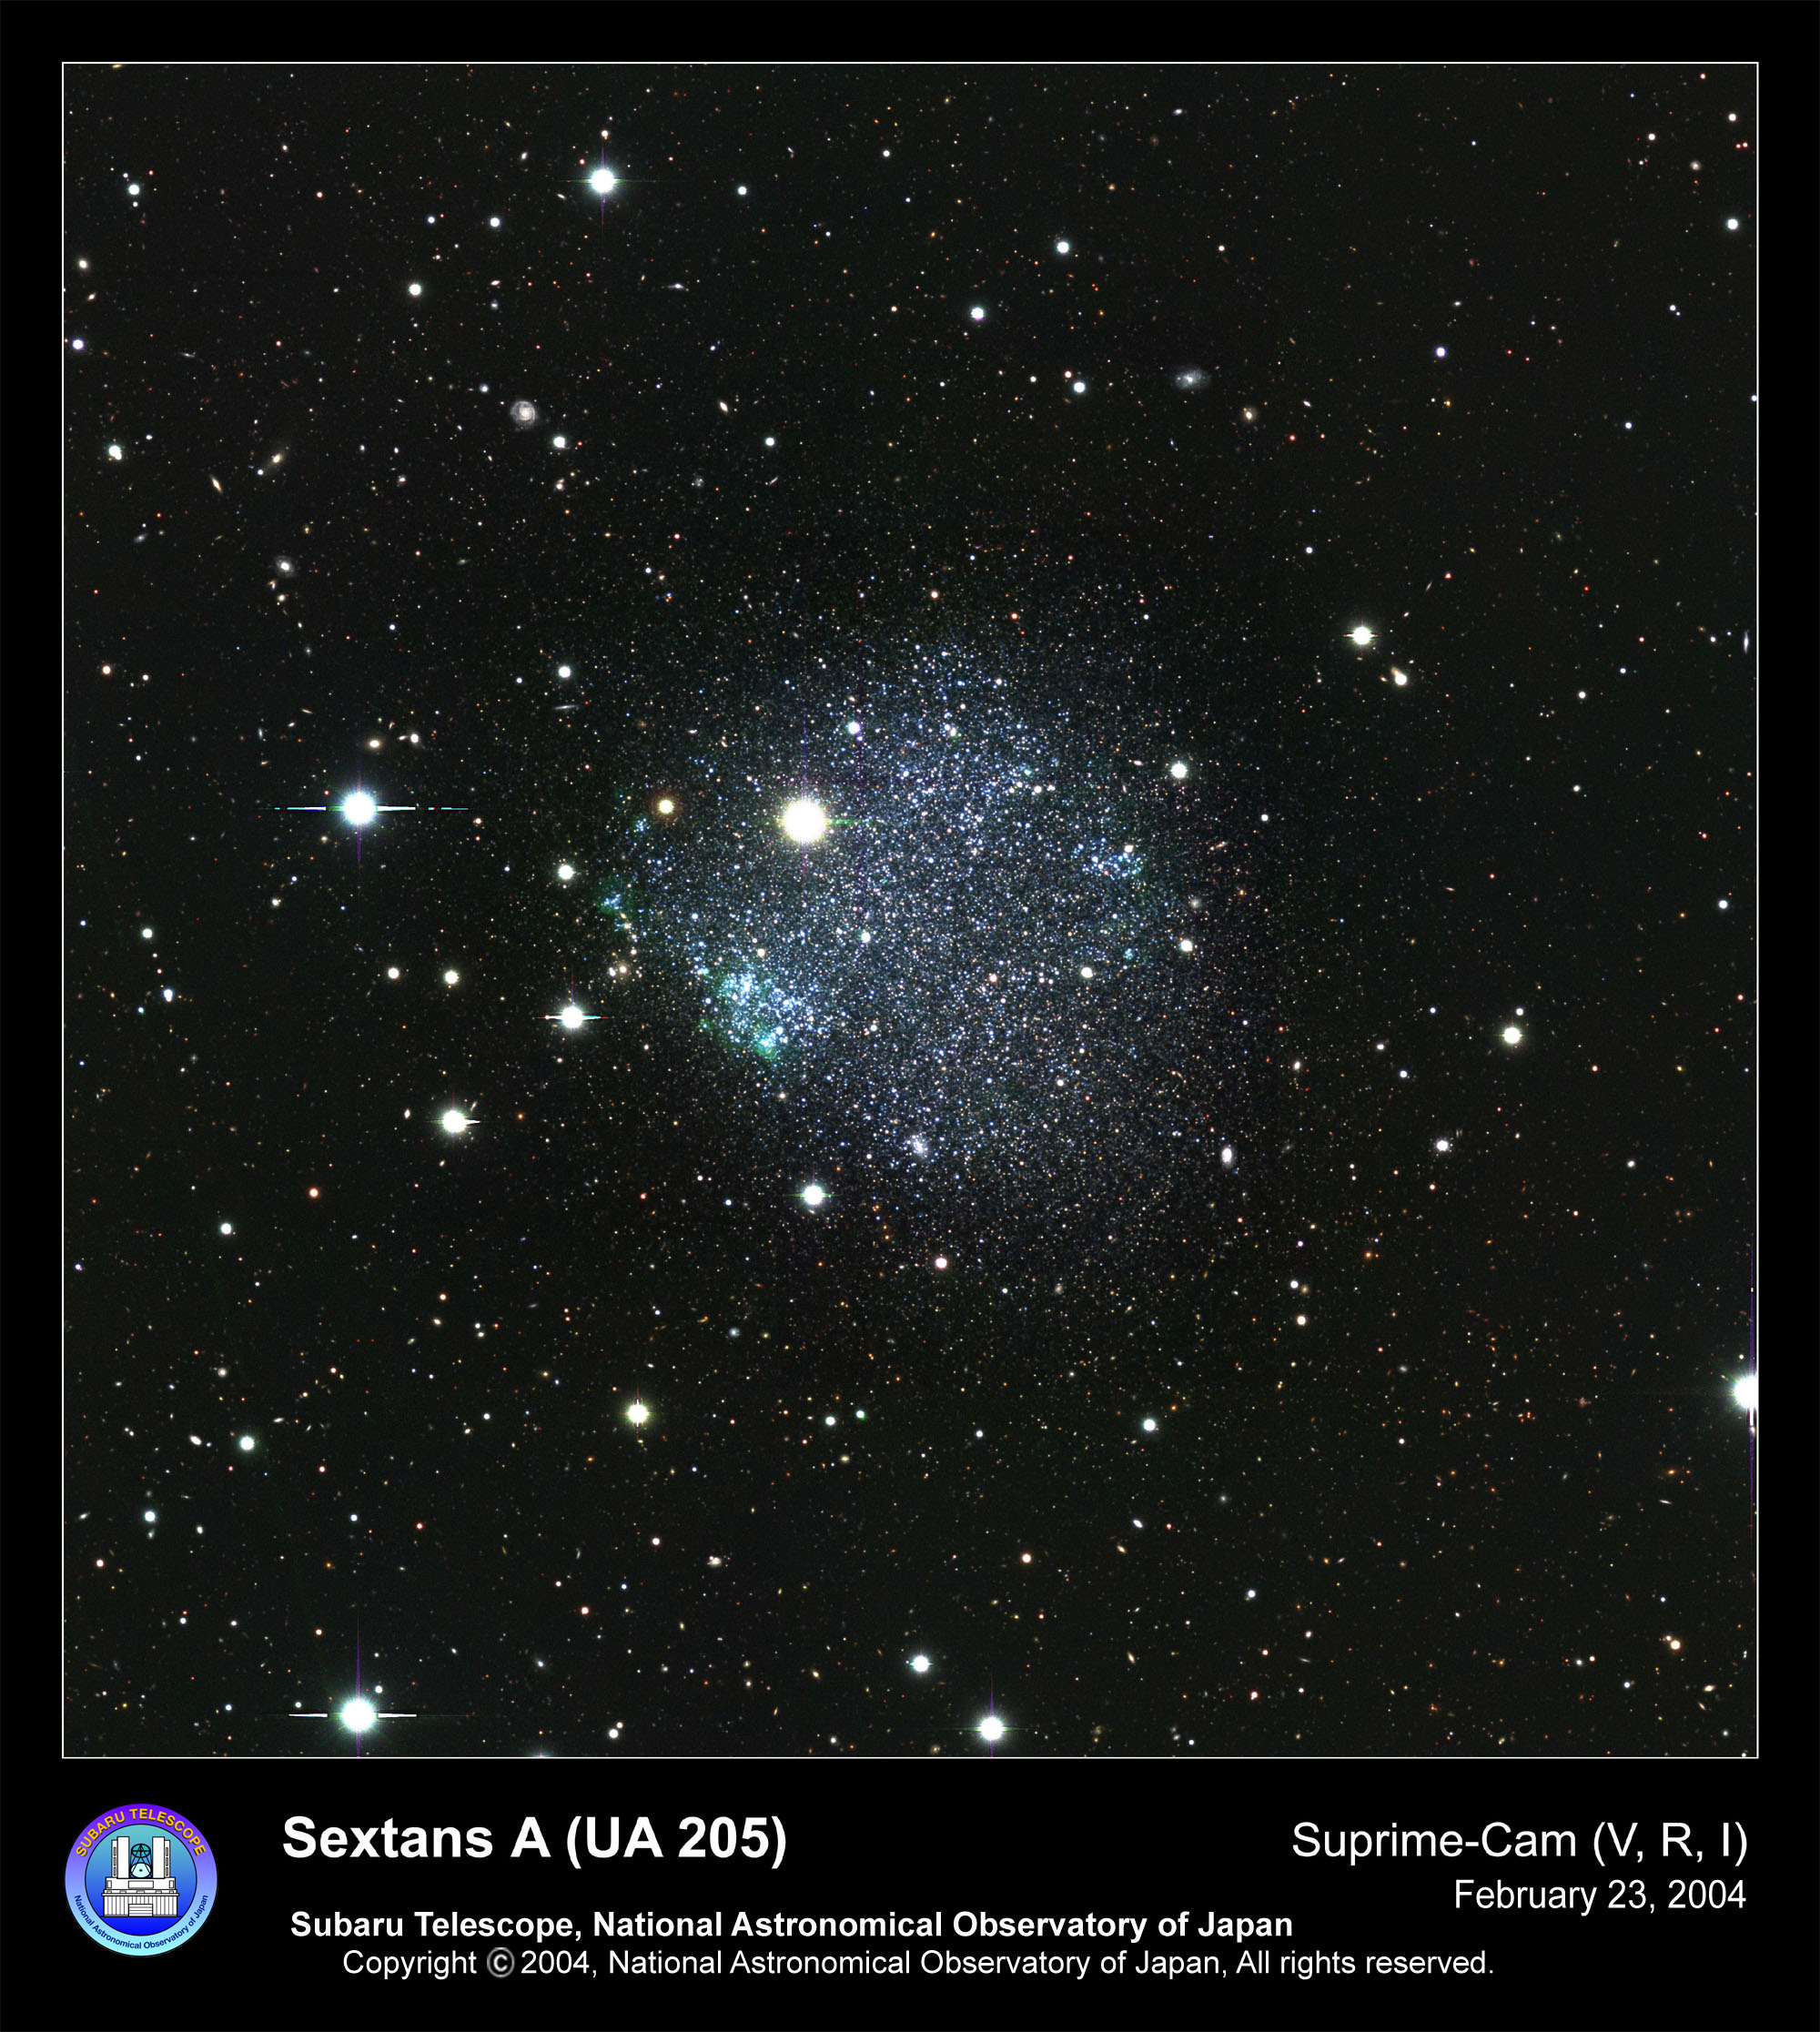
\includegraphics[width=0.58\textwidth]
{img/SextansA_300.jpg}

\caption{
Imagen compuesta de Sextans A obtenida con Suprime-Cam en el telescopio Subaru. La composición combina observaciones en los filtros $V$, $R$ e $I$, asociados a los canales azul, verde y rojo, respectivamente. La imagen muestra poblaciones estelares jóvenes de color azul, poblaciones más evolucionadas de tonos amarillos y rojos, y regiones asociadas a gas ionizado por estrellas masivas jóvenes \citep{subaru2004sextansa}.
}

\label{fig:sextansa_subaru}

\end{figure}

Desde el punto de vista físico, Sextans A es un ejemplo representativo de galaxia enana irregular. Estos sistemas no presentan la simetría global característica de galaxias espirales o elípticas, y suelen estar dominados por poblaciones jóvenes, gas interestelar y formación estelar reciente. La masa estelar de Sextans A es mucho menor que la de la Vía Láctea; la descripción de Subaru la compara con un sistema de aproximadamente $10^8$ estrellas, cerca de una milésima de la masa estelar de nuestra galaxia \citep{subaru2004sextansa}. Esta baja masa hace que su evolución sea sensible a procesos locales como la retroalimentación de estrellas masivas, la distribución del gas y la pérdida o retención de material enriquecido.

Sextans A es particularmente interesante porque su baja metalicidad permite estudiar poblaciones estelares en un ambiente químicamente distinto al de la vecindad solar. Observaciones con el Telescopio Espacial Hubble han permitido resolver estrellas individuales y construir diagramas color--magnitud utilizados para reconstruir la historia reciente de formación estelar de la galaxia \citep{dohmpalmer2002}. Trabajos recientes la describen como un sistema de muy baja metalicidad, del orden de $0.1\,Z_{\odot}$, con una población de estrellas masivas que puede estudiarse mediante fotometría ultravioleta de HST \citep{flores2026}.

La imagen de la Fig.~\ref{fig:sextansa_subaru} también ilustra la relación entre población estelar y medio interestelar. Según la descripción de Subaru, la región central contiene una concentración importante de hidrógeno neutro, que funciona como reservorio para la formación de nuevas estrellas. Las estrellas azules trazan poblaciones jóvenes y calientes, mientras que las regiones verdosas corresponden a gas ionizado en regiones HII por la radiación de esas estrellas jóvenes \citep{subaru2004sextansa}. Observaciones de radio muestran, además, que el hidrógeno neutro puede extenderse más allá de la zona donde la luz estelar de la galaxia se vuelve débil, lo cual plantea preguntas sobre el origen del gas y su efecto en la formación estelar.

En términos observacionales, la imagen de Subaru fue obtenida el 11 de noviembre de 2002 con exposiciones de $35$ min en $V$, $14$ min en $R$ y $24$ min en $I$. El campo de visión reportado es de aproximadamente $13.3^{\prime}\times13.3^{\prime}$, con el norte hacia arriba y el este hacia la izquierda, centrado cerca de $\alpha_{\rm J2000}=10^{\rm h}11^{\rm m}1.3^{\rm s}$ y $\delta_{\rm J2000}=-4^{\circ}42^{\prime}48^{\prime\prime}$ \citep{subaru2004sextansa}. Estos datos son relevantes porque conectan la apariencia de la galaxia con decisiones prácticas de fotometría: escala angular, profundidad de exposición, bandas usadas y separación entre poblaciones estelares.

Desde el punto de vista metodológico, Sextans A representa un caso útil para extender los procedimientos desarrollados en este trabajo. La detección de fuentes, la selección del radio de apertura, la estimación del fondo local y la construcción de CMDs siguen siendo etapas relevantes, pero se aplican en un régimen observacional distinto. Al tratarse de un objeto extragaláctico, las estrellas resueltas son más débiles y la contaminación por fuentes cercanas, la extinción, la calibración fotométrica y la posible necesidad de fotometría de PSF adquieren mayor importancia.

Por esta razón, el flujo desarrollado para M92 y M41 constituye una base para iniciar el análisis de Sextans A. En particular, los criterios de aislamiento mediante vecinos cercanos y de contaminación del anillo de cielo pueden ser adaptados para evaluar la calidad de la fotometría en campos donde la separación entre fuentes y la estimación del fondo influyen directamente en la confiabilidad de las magnitudes instrumentales.


% ============================================================
% IRAF
% ============================================================

\subsection{IRAF}

IRAF, \textit{Image Reduction and Analysis Facility}, es un entorno de software desarrollado para el procesamiento y análisis de datos astronómicos.

IRAF organiza sus herramientas mediante paquetes y tareas.

Entre los paquetes utilizados en este trabajo se encuentran

En este trabajo se utilizaron los paquetes \texttt{images}, \texttt{noao}, \texttt{imred}, \texttt{ccdred}, \texttt{digiphot} y \texttt{apphot}, seleccionados de acuerdo con las etapas de reducción, inspección y fotometría desarrolladas.

Entre las tareas empleadas se encuentran

Las tareas empleadas fueron \texttt{imhead}, \texttt{display}, \texttt{imexamine}, \texttt{ccdproc}, \texttt{imcopy}, \texttt{daofind}, \texttt{tvmark}, \texttt{qphot}, \texttt{phot} y \texttt{txdump}. Cada una se utilizó en una etapa específica del flujo de trabajo, desde la inspección inicial de los encabezados FITS hasta la extracción final de coordenadas, magnitudes y errores fotométricos.


% ============================================================
% DAOFIND
% ============================================================

\subsection{Detección automática mediante \texttt{daofind}}

La tarea \texttt{daofind} permite identificar automáticamente fuentes aproximadamente estelares.

Para realizar la detección utiliza información sobre la forma esperada de las fuentes y sobre el nivel de ruido del fondo.

Dos parámetros fundamentales son

Entre los parámetros fundamentales de \texttt{daofind} se encuentran \texttt{fwhmpsf}, que describe el tamaño característico de las fuentes, y \texttt{threshold}, que establece el umbral de detección respecto al nivel de ruido del fondo.

El parámetro \texttt{threshold}, denominado umbral de detección, representa un límite expresado en unidades relacionadas con el ruido del fondo.

Un valor demasiado pequeño puede producir numerosas falsas detecciones.

Un valor excesivamente grande puede eliminar estrellas débiles reales.

Por ello la selección debe realizarse estudiando simultáneamente el número de detecciones y su distribución visual sobre la imagen.


% ============================================================
% CAPÍTULO 2
% METODOLOGÍA
% ============================================================


% ============================================================
% ESTRUCTURA DEL DOCUMENTO
% ============================================================

\section{Estructura del documento}

El presente capítulo reúne la contextualización del problema, los fundamentos teóricos necesarios para comprender el funcionamiento de los detectores CCD, las principales fuentes de ruido, los procedimientos de calibración, la formación de la imagen estelar, la fotometría de apertura, los criterios de selección de fuentes y los diagramas color--magnitud. Al final del capítulo se presentan la pregunta de investigación y los objetivos que orientan el trabajo.

El Capítulo 2 describe la metodología empleada para la reducción de las imágenes de M92 y el análisis fotométrico de M92 y M41. El Capítulo 3 reúne los resultados obtenidos y su discusión, relacionando los procedimientos aplicados con el comportamiento observado en las imágenes y en las mediciones fotométricas. El Capítulo 4 presenta las conclusiones y las posibles líneas de trabajo futuro.

\section{Pregunta de investigación}

¿Cómo se puede implementar un flujo de trabajo basado en IRAF que permita reducir imágenes CCD, identificar y seleccionar fuentes estelares y obtener magnitudes instrumentales confiables mediante fotometría de apertura en imágenes de los cúmulos M92 y M41?


\section{Objetivos}

\subsection{Objetivo general}

Implementar un flujo de trabajo para la reducción de imágenes CCD, identificación de fuentes y obtención de magnitudes instrumentales mediante fotometría de apertura utilizando IRAF, aplicado a observaciones de M92 y M41.


\subsection{Objetivos específicos}

El primer objetivo específico consiste en aplicar procedimientos de reducción CCD a imágenes de M92, incluyendo la inspección de encabezados, la corrección por \textit{overscan}, el recorte de la región científica, la corrección por \textit{bias} y la corrección por \textit{flat field}.

El segundo objetivo específico es determinar parámetros adecuados para la detección y la fotometría de fuentes estelares mediante el análisis del FWHM, el fondo de cielo, el umbral de detección y el radio de apertura.

El tercer objetivo específico consiste en obtener y depurar magnitudes instrumentales de estrellas de M92 y M41 mediante fotometría de apertura, y evaluar los resultados a partir de los errores fotométricos, los criterios de aislamiento y los diagramas color--magnitud.


\chapter{Metodología}


% ============================================================
% DATOS
% ============================================================

\section{Datos utilizados}

El conjunto principal corresponde a imágenes CCD de M92 obtenidas en diferentes filtros.

Las imágenes utilizadas fueron:

\begin{table}[H]

\centering

\begin{tabular}{lll}

\toprule
Archivo & Objeto & Uso principal \\

\midrule

\texttt{m92010.fits} & M92 & Reducción y fotometría \\

\texttt{m92011.fits} & M92 & Reducción, fotometría y CMD \\

\texttt{m92014.fits} & M92 & Reducción y fotometría \\

\texttt{m92015.fits} & M92 & Reducción, fotometría y CMD \\

\texttt{M41.fits} & M41 & Fotometría multicanal \\

\bottomrule

\end{tabular}

\caption{Imágenes principales empleadas durante el análisis.}

\label{tab:datos}

\end{table}


% ============================================================
% ENTORNO
% ============================================================

\section{Entorno computacional}

El procesamiento se realizó principalmente mediante IRAF.

La visualización de imágenes y el marcado interactivo de coordenadas se realizó mediante un servidor gráfico compatible con las tareas \texttt{display} y \texttt{tvmark}.

Python fue utilizado adicionalmente para realizar análisis numérico, procesamiento de los archivos producidos por IRAF, comparación de coordenadas, análisis estadístico y generación de gráficas.


% ============================================================
% REDUCCIÓN
% ============================================================

\section{Reducción CCD de M92}

El primer procedimiento consistió en inspeccionar los encabezados FITS de \texttt{m92010.fits}, \texttt{m92011.fits}, \texttt{m92014.fits} y \texttt{m92015.fits} mediante la tarea \texttt{imhead} con la opción \texttt{long+}. Esta inspección permitió revisar la información contenida en los encabezados antes de modificar los archivos y reconocer los parámetros necesarios para la reducción.

Posteriormente se cargaron los paquetes \texttt{noao}, \texttt{imred} y \texttt{ccdred}, y se configuró la tarea \texttt{ccdproc} mediante \texttt{epar}. El procedimiento de reducción consideró de manera secuencial la corrección de la región de sobrelectura (\textit{overscan}), el recorte de la región científica, la corrección del nivel de polarización (\textit{bias}) y la corrección de campo plano (\textit{flat field}), de acuerdo con la estructura particular de las imágenes utilizadas.


% ============================================================
% IDENTIFICACIÓN MANUAL
% ============================================================

\section{Identificación manual de estrellas}

Las imágenes fueron visualizadas mediante \texttt{display}; por ejemplo, \texttt{m92011.fits} se cargó en el marco gráfico y posteriormente se examinó de forma interactiva con \texttt{imexamine}. Durante esta inspección se seleccionaron estrellas relativamente brillantes, no saturadas y preferiblemente aisladas, y se utilizaron sus perfiles radiales para estimar el FWHM. También se examinaron regiones representativas del cielo con el fin de caracterizar el nivel y la dispersión del fondo.


% ============================================================
% FWHM
% ============================================================

\section{Determinación del FWHM}

Para cada imagen se midió el FWHM de múltiples estrellas.

Posteriormente se calculó la mediana.

Se eligió la mediana porque es menos sensible que la media a valores atípicos provocados por fuentes saturadas, mezcladas o con perfiles anómalos.


% ============================================================
% APERTURAS
% ============================================================

\section{Selección de apertura y umbral de detección}

Se adoptó como radio de apertura $r_{\rm ap}=3\,{\rm median}(FWHM)$. Los valores utilizados para cada imagen se resumen en la Tabla~\ref{tab:fwhm}:

\begin{table}[H]

\centering

\begin{tabular}{lccc}

\toprule

Imagen &
Mediana FWHM [pix] &
$3\times FWHM$ [pix] &
Threshold \\

\midrule

\texttt{m92010.fits} & 2.900 & 8.700 & 3.5 \\

\texttt{m92011.fits} & 3.355 & 10.065 & 3.5 \\

\texttt{m92014.fits} & 3.295 & 9.885 & 3.5 \\

\texttt{m92015.fits} & 3.025 & 9.075 & 3.5 \\

\texttt{M41.fits} & 2.220 & 6.660 & 3.5 \\

\bottomrule

\end{tabular}

\caption{
Valores de FWHM, radio de apertura y threshold utilizados durante el análisis.
}

\label{tab:fwhm}

\end{table}


% ============================================================
% M41
% ============================================================

\section{Procesamiento de M41}

El archivo \texttt{M41.fits} estaba compuesto por múltiples extensiones FITS. Cada extensión, identificada como \texttt{M41.fits[0]}, \texttt{M41.fits[1]} y \texttt{M41.fits[2]}, fue inspeccionada mediante \texttt{imhead} con la opción \texttt{long+} para verificar su contenido y reconocer el canal asociado. Después de esta revisión se utilizó \texttt{imcopy} para extraer cada extensión y almacenarla como una imagen independiente, generando los archivos \texttt{M41\_blue.fits}, \texttt{M41\_red.fits} y \texttt{M41\_green.fits}. De esta manera fue posible trabajar de forma separada con los tres canales durante las etapas posteriores del análisis.


% ============================================================
% DETECCIÓN
% ============================================================

\section{Detección automática de estrellas}

La detección automática se realizó mediante \texttt{daofind}. Para cada imagen se especificó el archivo de salida de coordenadas, el valor de \texttt{fwhmpsf} determinado previamente a partir del FWHM, la dispersión del fondo mediante el parámetro \texttt{sigma} y un umbral de detección de \texttt{threshold=3.5}; además, se desactivó la verificación interactiva con \texttt{verify-}. Las coordenadas generadas fueron posteriormente superpuestas sobre la imagen con \texttt{tvmark}, lo que permitió comprobar visualmente que las detecciones correspondieran a fuentes estelares reales y descartar posibles identificaciones espurias.


% ============================================================
% PHOT
% ============================================================

\section{Fotometría de apertura}

Después de determinar las coordenadas, las magnitudes instrumentales fueron obtenidas mediante \texttt{phot}. Para cada imagen se indicó el archivo de coordenadas correspondiente y se definió un archivo de salida con extensión \texttt{.mag}; las opciones \texttt{interac-} y \texttt{verify-} permitieron ejecutar el procedimiento sin interacción manual para cada fuente. Una vez finalizada la fotometría, la tarea \texttt{txdump} se utilizó para extraer de los archivos resultantes las columnas \texttt{XCENTER}, \texttt{YCENTER}, \texttt{MAG} y \texttt{MERR}, que contienen las coordenadas de las fuentes, sus magnitudes instrumentales y los errores fotométricos. Estos valores se guardaron en archivos de texto para realizar los análisis numéricos y las gráficas posteriores.


% ============================================================
% CMD
% ============================================================

\section{Construcción del CMD de M92}

Para construir el diagrama color--magnitud se utilizaron las mediciones de las imágenes

Para construir el diagrama color--magnitud se utilizaron las mediciones de \texttt{m92011.fits}, correspondiente al filtro $V$, y de \texttt{m92015.fits}, correspondiente al filtro $B$.

Para cada estrella presente en ambos conjuntos se calculó el color instrumental como $(B-V)_i=B_i-V_i$ y posteriormente se construyó el diagrama $(B-V)$ frente a $V$. El eje correspondiente a $V$ fue invertido para conservar la convención astronómica según la cual las magnitudes menores representan objetos más brillantes.


% ============================================================
% VECINOS
% ============================================================

\section{Filtro de vecinos más cercanos}

Después de obtener las coordenadas de las estrellas se calculó, para cada una, la distancia hasta todas las demás fuentes.

La distancia mínima fue utilizada como distancia al vecino más cercano.

Para \texttt{m92011.fits} se utilizó un $FWHM=3.355\ {\rm pix}$, por lo que el límite de $3FWHM$ correspondió a $10.065\ {\rm pix}$. Se descartó una fuente cuando la distancia a su vecino más cercano cumplía $d_{\rm vecino}\leq10.065\ {\rm pix}$. Las listas resultantes fueron posteriormente marcadas mediante \texttt{tvmark} para inspeccionar visualmente la clasificación.


% ============================================================
% CIELO
% ============================================================

\section{Análisis de contaminación del anillo de cielo}

Como segundo criterio de calidad se analizaron los píxeles contenidos dentro del anillo de cielo de cada estrella.

Se utilizó un radio interno de $r_{\rm in}=15\ {\rm pix}$ y un ancho de $\Delta r=10\ {\rm pix}$, de modo que el anillo de cielo abarcó el intervalo $15\leq r\leq25\ {\rm pix}$. Se estudió la distribución de los valores de los píxeles dentro de cada anillo y se identificaron valores atípicos altos.

Una fracción elevada de estos valores puede indicar la presencia de otra fuente estelar dentro del anillo.

Las estrellas asociadas a anillos contaminados fueron descartadas de la muestra fotométrica final.


% ============================================================
% CAPÍTULO 3
% RESULTADOS
% ============================================================

\chapter{Resultados y discusión}


% ============================================================
% REDUCCIÓN RESULTADOS
% ============================================================

\section{Reducción CCD de M92}

La aplicación del proceso de reducción permitió transformar las imágenes originales de M92 en imágenes preparadas para los procedimientos fotométricos posteriores.

La comparación visual entre imágenes crudas y reducidas permitió verificar la modificación de las regiones correspondientes al overscan y el recorte de la región científica.

\begin{figure}[H]

\centering

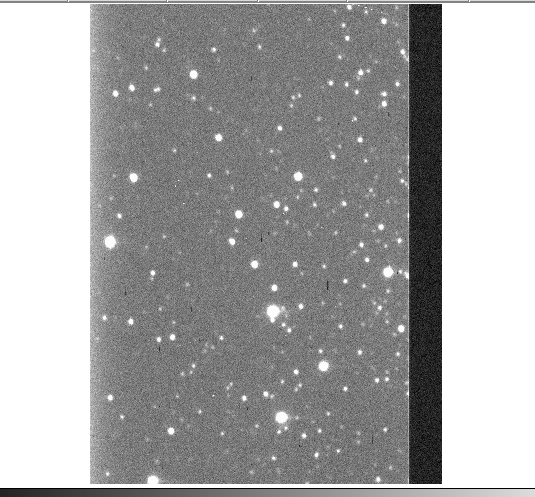
\includegraphics[width=0.65\textwidth]
{img/Screenshot From 2026-07-06 14-04-23.png}

\caption{
Imagen cruda correspondiente a \texttt{m92010.fits}.
}

\label{fig:m92010raw}

\end{figure}


\begin{figure}[H]

\centering

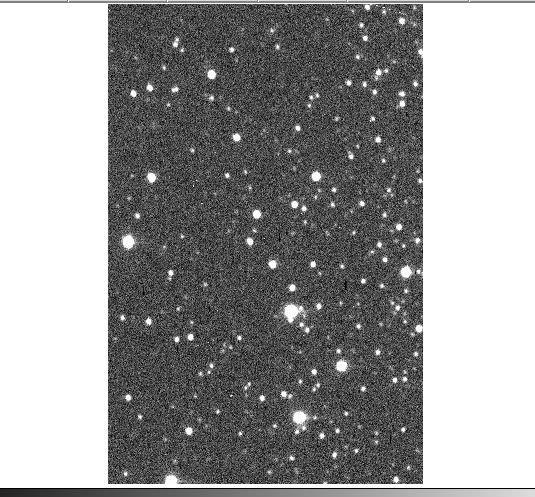
\includegraphics[width=0.65\textwidth]
{img/Screenshot From 2026-07-06 14-06-10.png}

\caption{
Imagen \texttt{m92010.fits} después del proceso de reducción.
}

\label{fig:m92010reducida}

\end{figure}


% ============================================================
% M41 RESULTADOS
% ============================================================

\section{Separación de canales de M41}

La estructura multiextensión de M41 fue separada en tres imágenes independientes.

\begin{figure}[H]

\centering

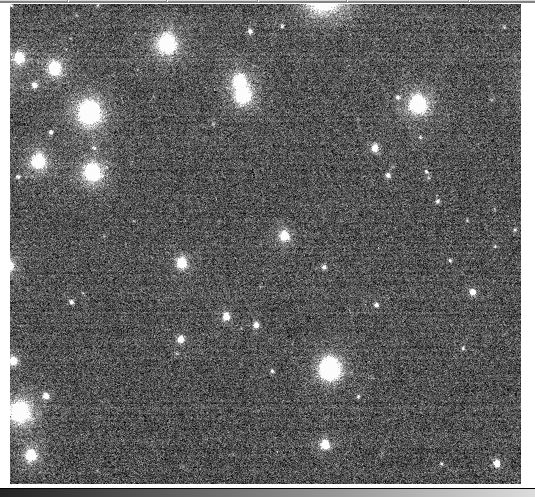
\includegraphics[width=0.55\textwidth]
{img/Screenshot From 2026-07-06 14-13-44.png}

\caption{Canal azul del archivo M41.}

\label{fig:m41blue}

\end{figure}


\begin{figure}[H]

\centering

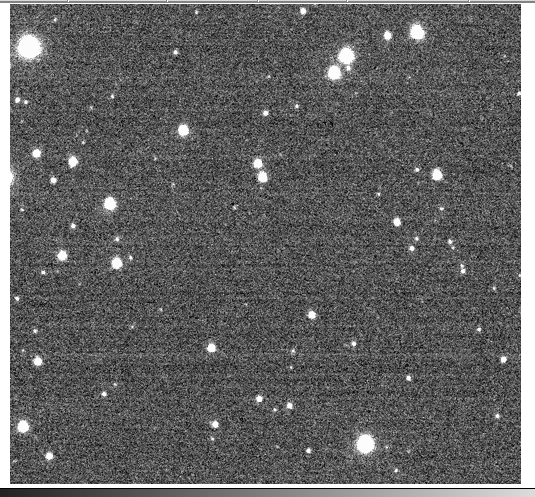
\includegraphics[width=0.55\textwidth]
{img/Screenshot From 2026-07-06 14-13-55.png}

\caption{Canal rojo del archivo M41.}

\label{fig:m41red}

\end{figure}


\begin{figure}[H]

\centering

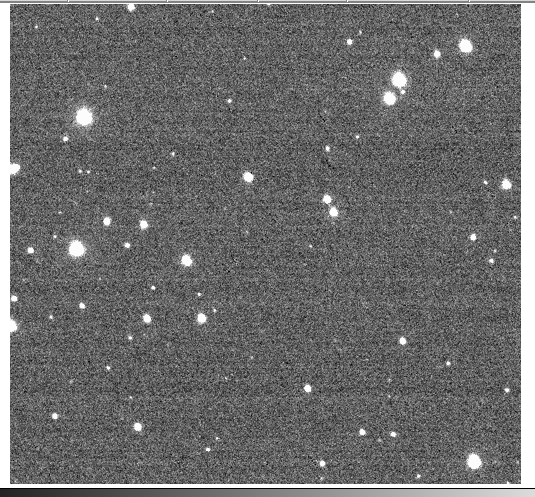
\includegraphics[width=0.55\textwidth]
{img/Screenshot From 2026-07-06 14-14-03.png}

\caption{Canal verde del archivo M41.}

\label{fig:m41green}

\end{figure}


% ============================================================
% THRESHOLD
% ============================================================

\section{Selección del umbral de detección}

Se estudiaron diferentes valores del umbral de detección con el objetivo de analizar cómo variaba el número de fuentes identificadas automáticamente.

El valor finalmente adoptado para el procedimiento fotométrico fue \texttt{threshold=3.5}, ya que permitió conservar una cantidad importante de detecciones evitando un aumento excesivo de fuentes espurias.


\begin{figure}[H]

\centering

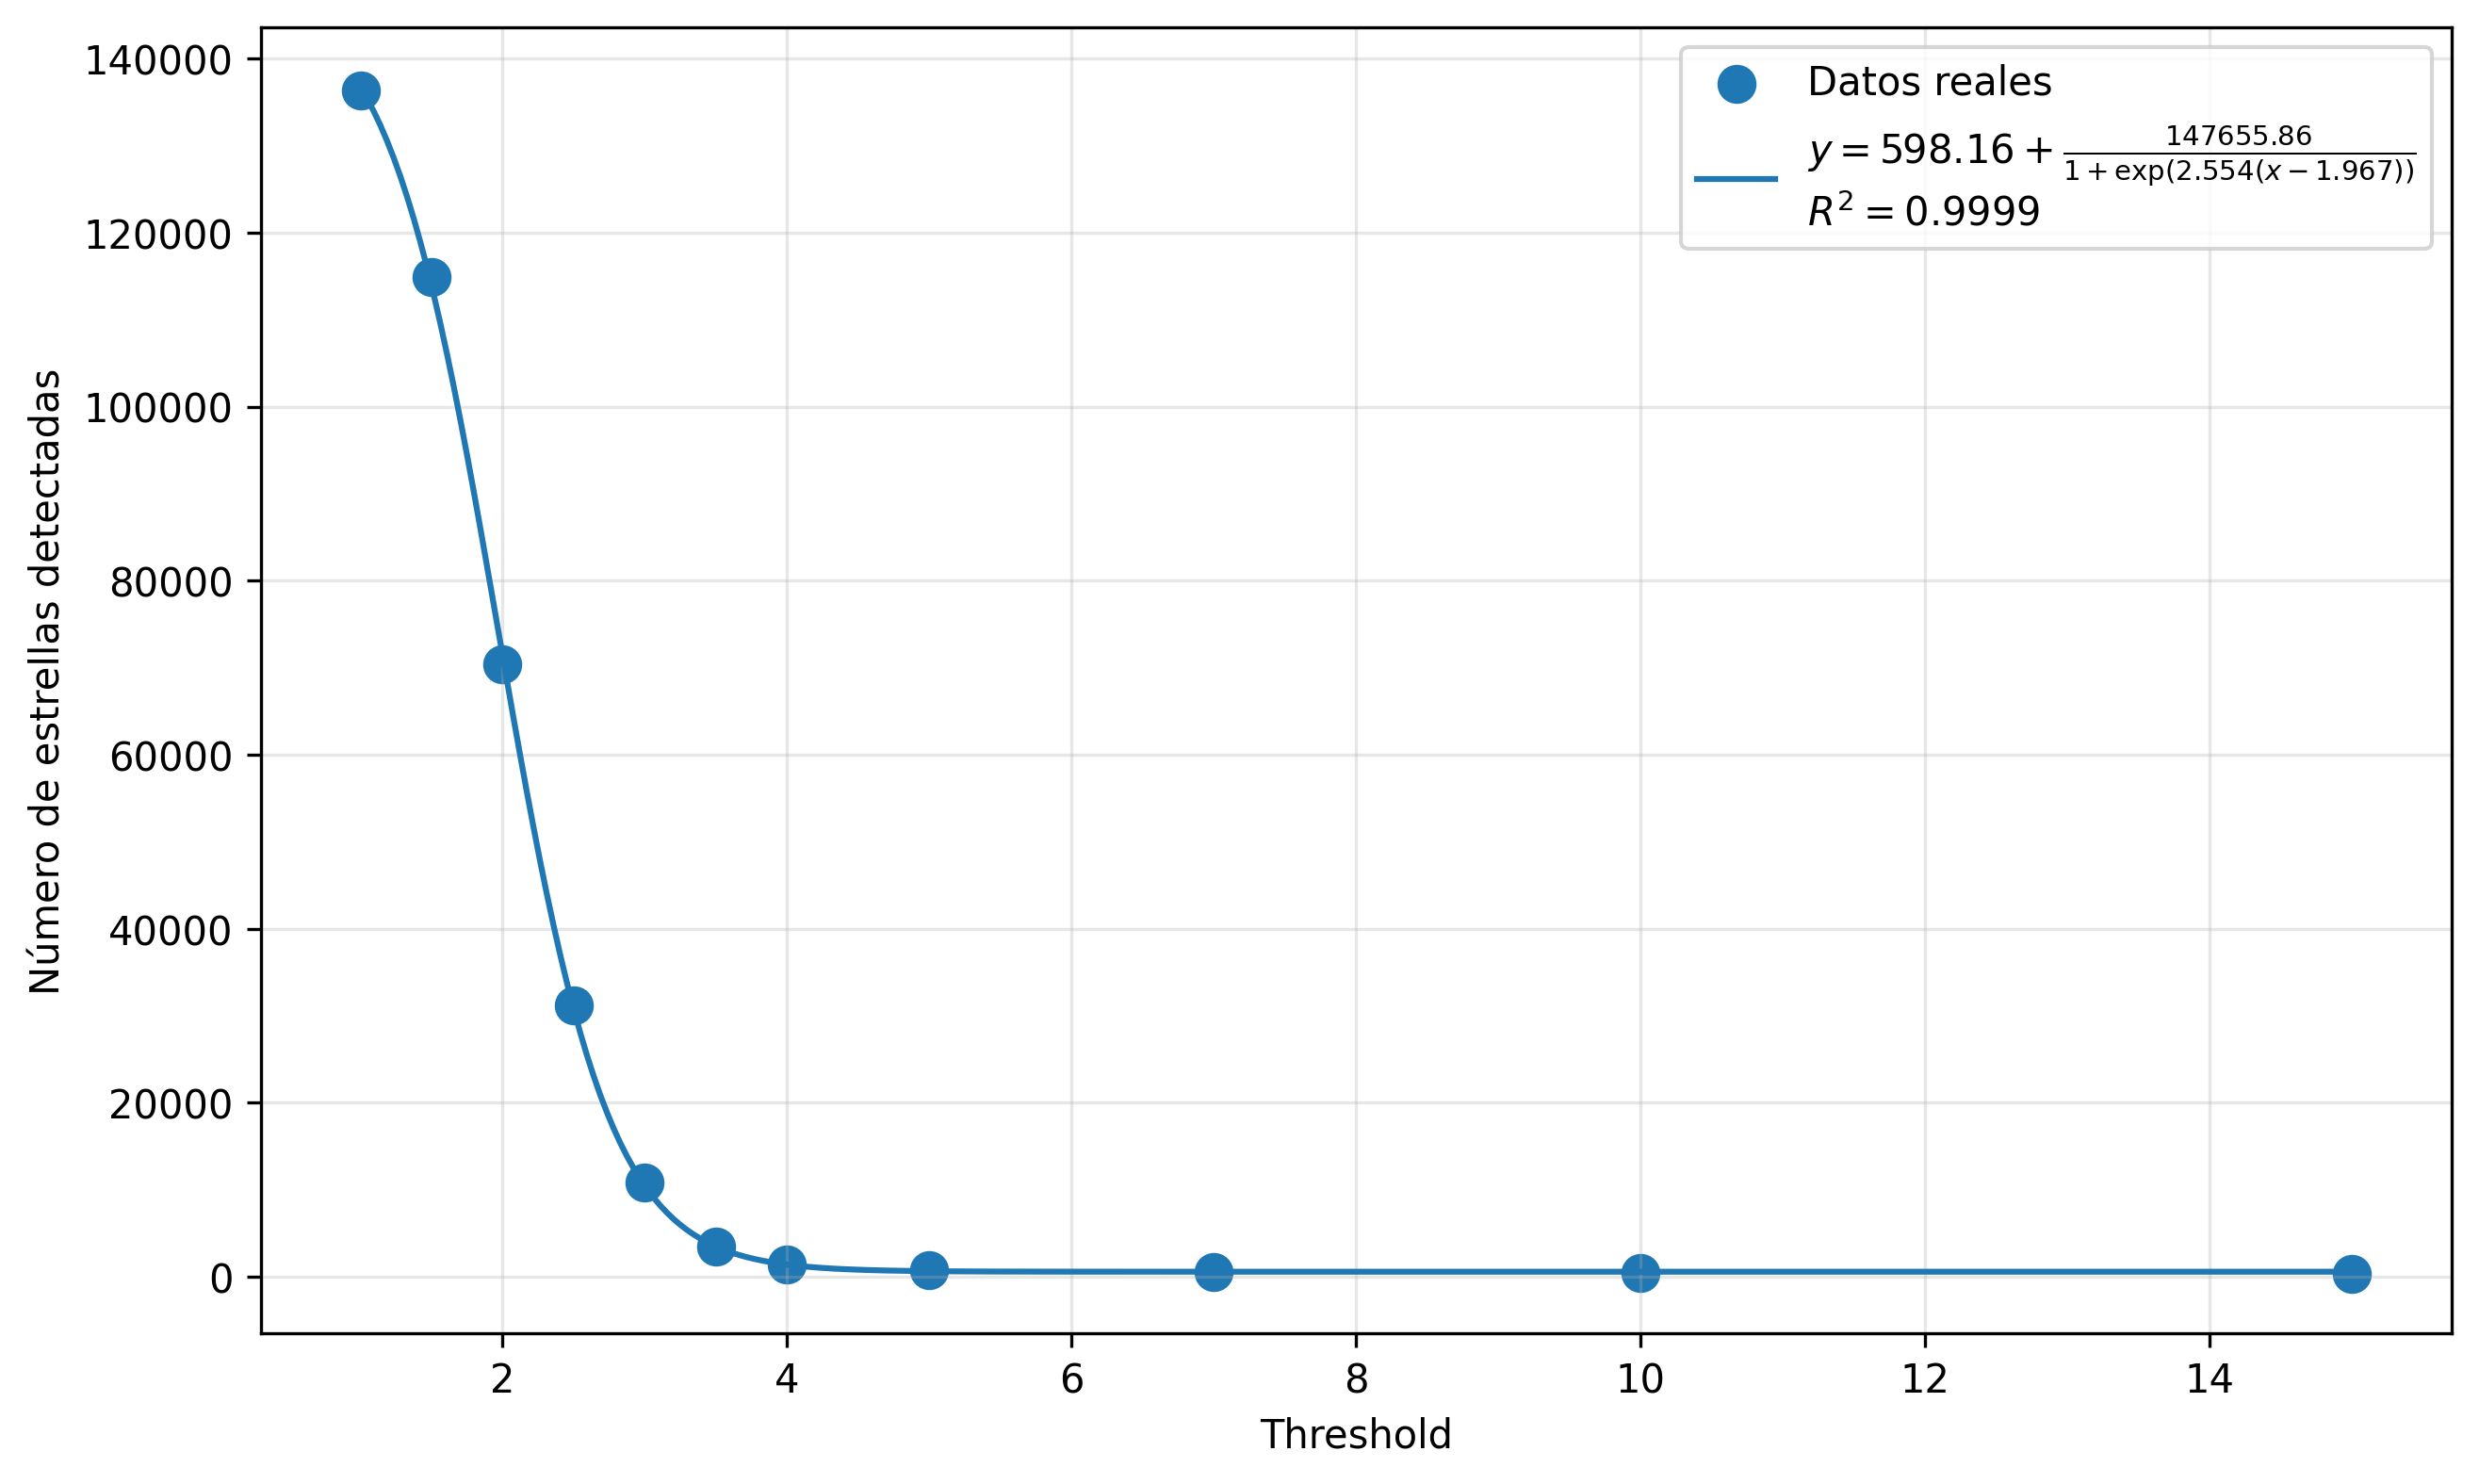
\includegraphics[width=0.85\textwidth]
{img/ajuste_logistico.png}

\caption{
Análisis utilizado para estudiar la variación del número de detecciones en función del umbral de detección. $y = 598.16 + \frac{147655.86}{1 + e^{2.554(x-1.967)}}$
}

\label{fig:threshold}

\end{figure}


% ============================================================
% ESTRELLAS M92
% ============================================================

\section{Detección automática en M92}

La tarea \texttt{daofind} produjo una lista automática de fuentes para \texttt{m92011.fits}.

Las posiciones fueron posteriormente superpuestas sobre la imagen para verificar visualmente la correspondencia entre las coordenadas y las fuentes estelares.

\begin{figure}[H]

\centering

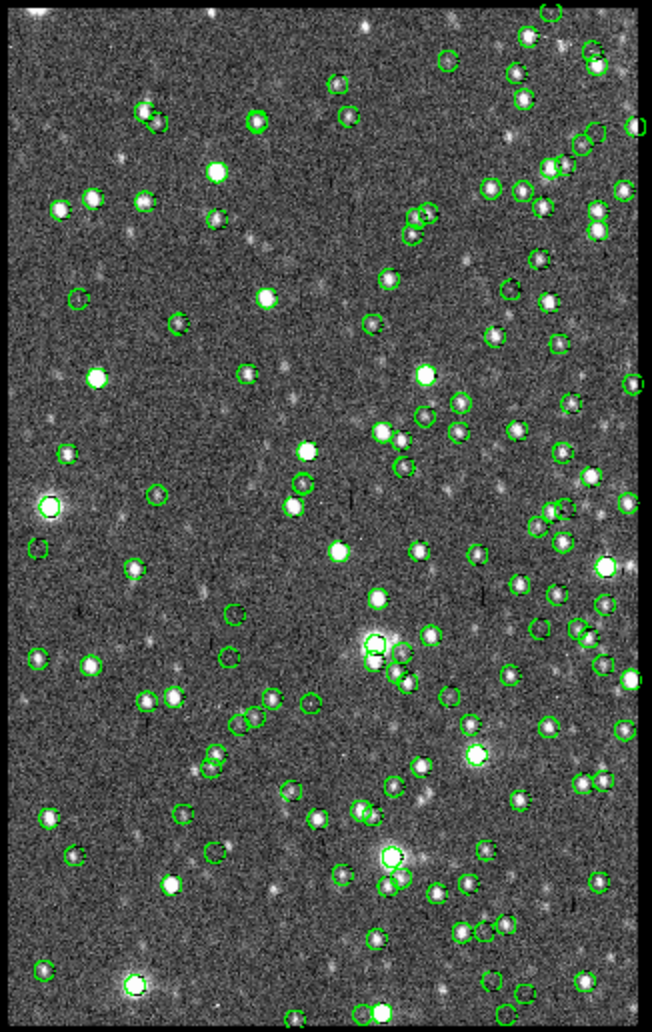
\includegraphics[width=0.60\textwidth]
{img/m92Encontradas}

\caption{
Estrellas detectadas automáticamente en \texttt{m92011.fits} utilizando \texttt{daofind} con un umbral de detección de 3.5.
}

\label{fig:m92011detecciones}

\end{figure}

% ============================================================
% ESTRELLAS M41
% ============================================================

\section{Detección automática en M41}

La tarea \texttt{daofind} se utilizó para realizar la detección automática de fuentes estelares en la imagen de M41. A partir de los parámetros previamente determinados para el FWHM, el nivel de ruido del fondo y el umbral de detección, se generó una lista de coordenadas correspondientes a las estrellas identificadas en el campo.

Posteriormente, las posiciones obtenidas fueron superpuestas sobre la imagen mediante \texttt{tvmark}, con el objetivo de verificar visualmente que las detecciones correspondieran a fuentes estelares reales y no a fluctuaciones del fondo o artefactos de la imagen.

\begin{figure}[H]

\centering

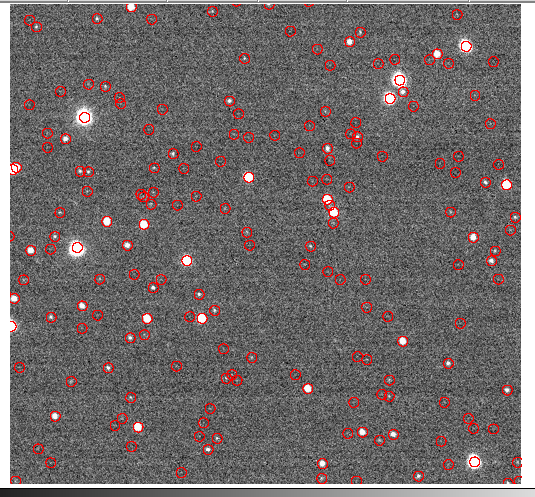
\includegraphics[width=0.60\textwidth]
{img/m41Encontradas.png}

\caption{
Estrellas detectadas automáticamente en M41 utilizando \texttt{daofind} y verificadas visualmente mediante \texttt{tvmark}.
}

\label{fig:m41detecciones}

\end{figure}


% ============================================================
% MAG MERR
% ============================================================

\section{Relación entre magnitud y error fotométrico}

Las magnitudes instrumentales obtenidas fueron comparadas con sus correspondientes errores fotométricos.

La tendencia esperada es un aumento del error hacia magnitudes mayores, debido a la disminución progresiva de la relación señal--ruido.


\begin{figure}[H]

\centering

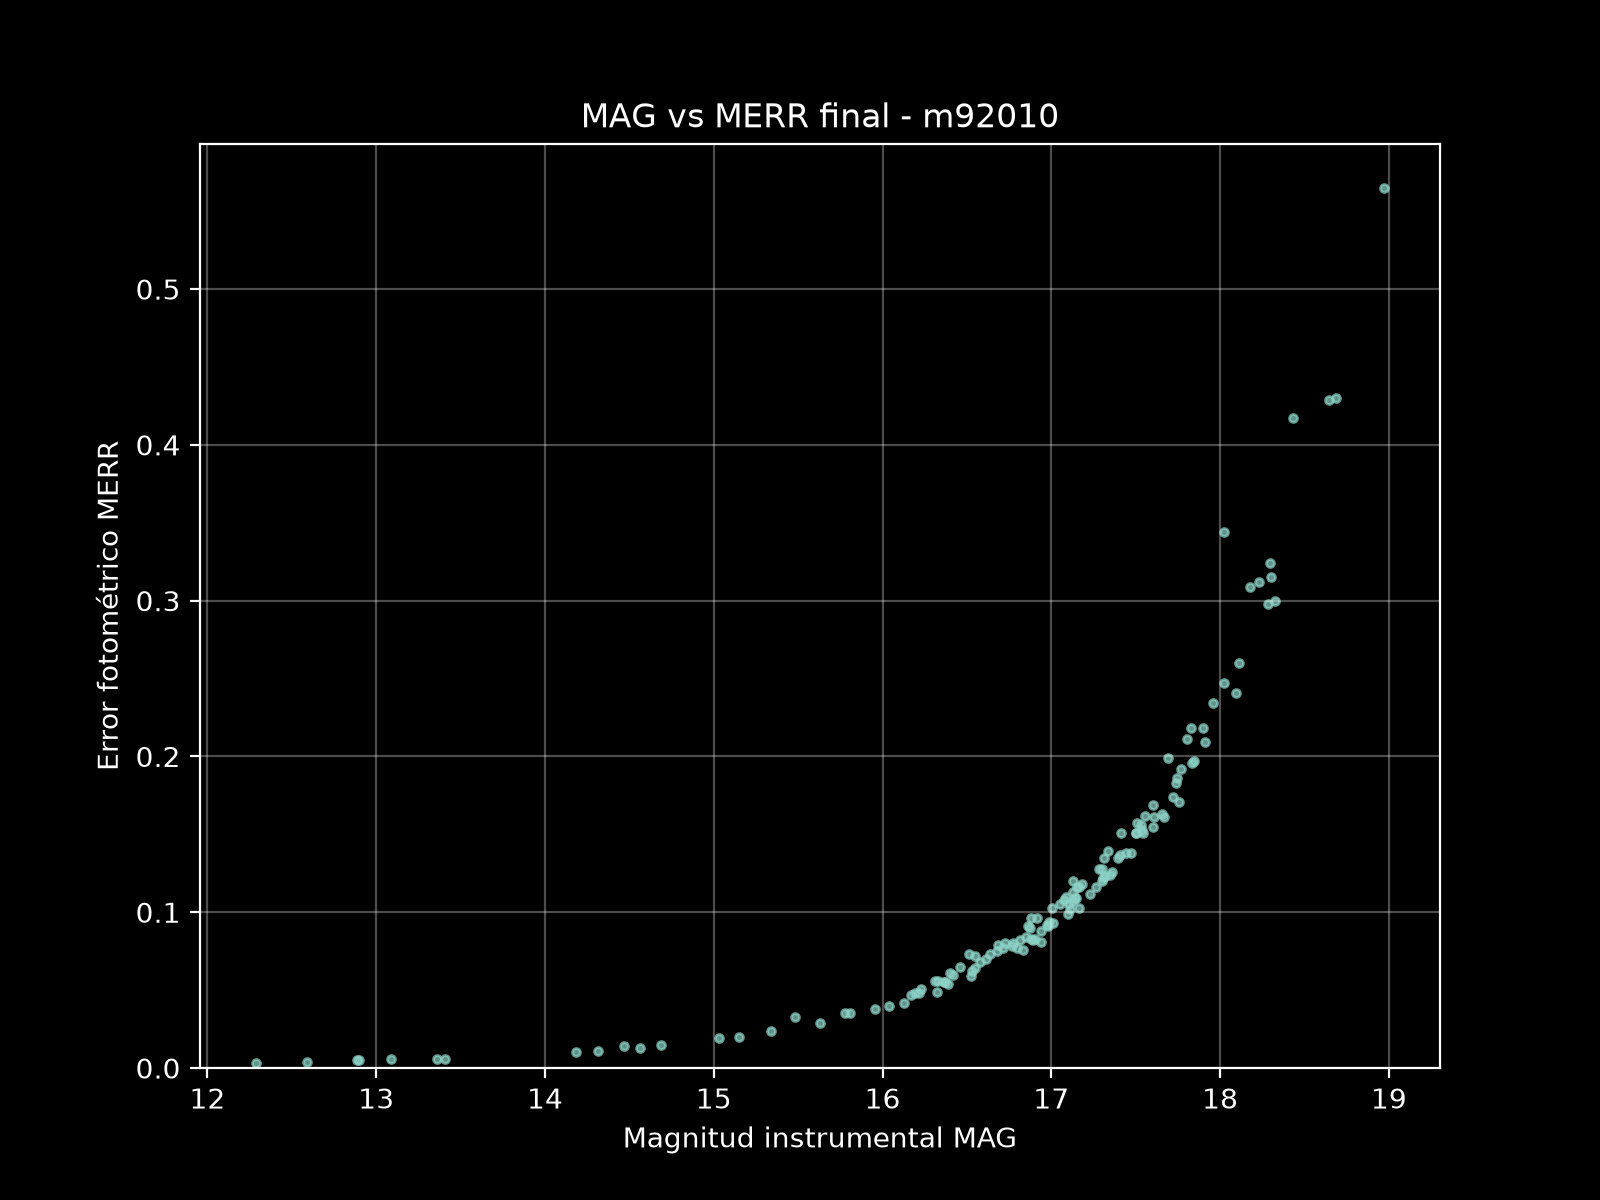
\includegraphics[width=0.65\textwidth]
{img/m92010_final_mag_vs_merr.png}

\caption{
Magnitud instrumental frente a error fotométrico para \texttt{m92010.fits}.
}

\label{fig:m92010merr}

\end{figure}


\begin{figure}[H]

\centering

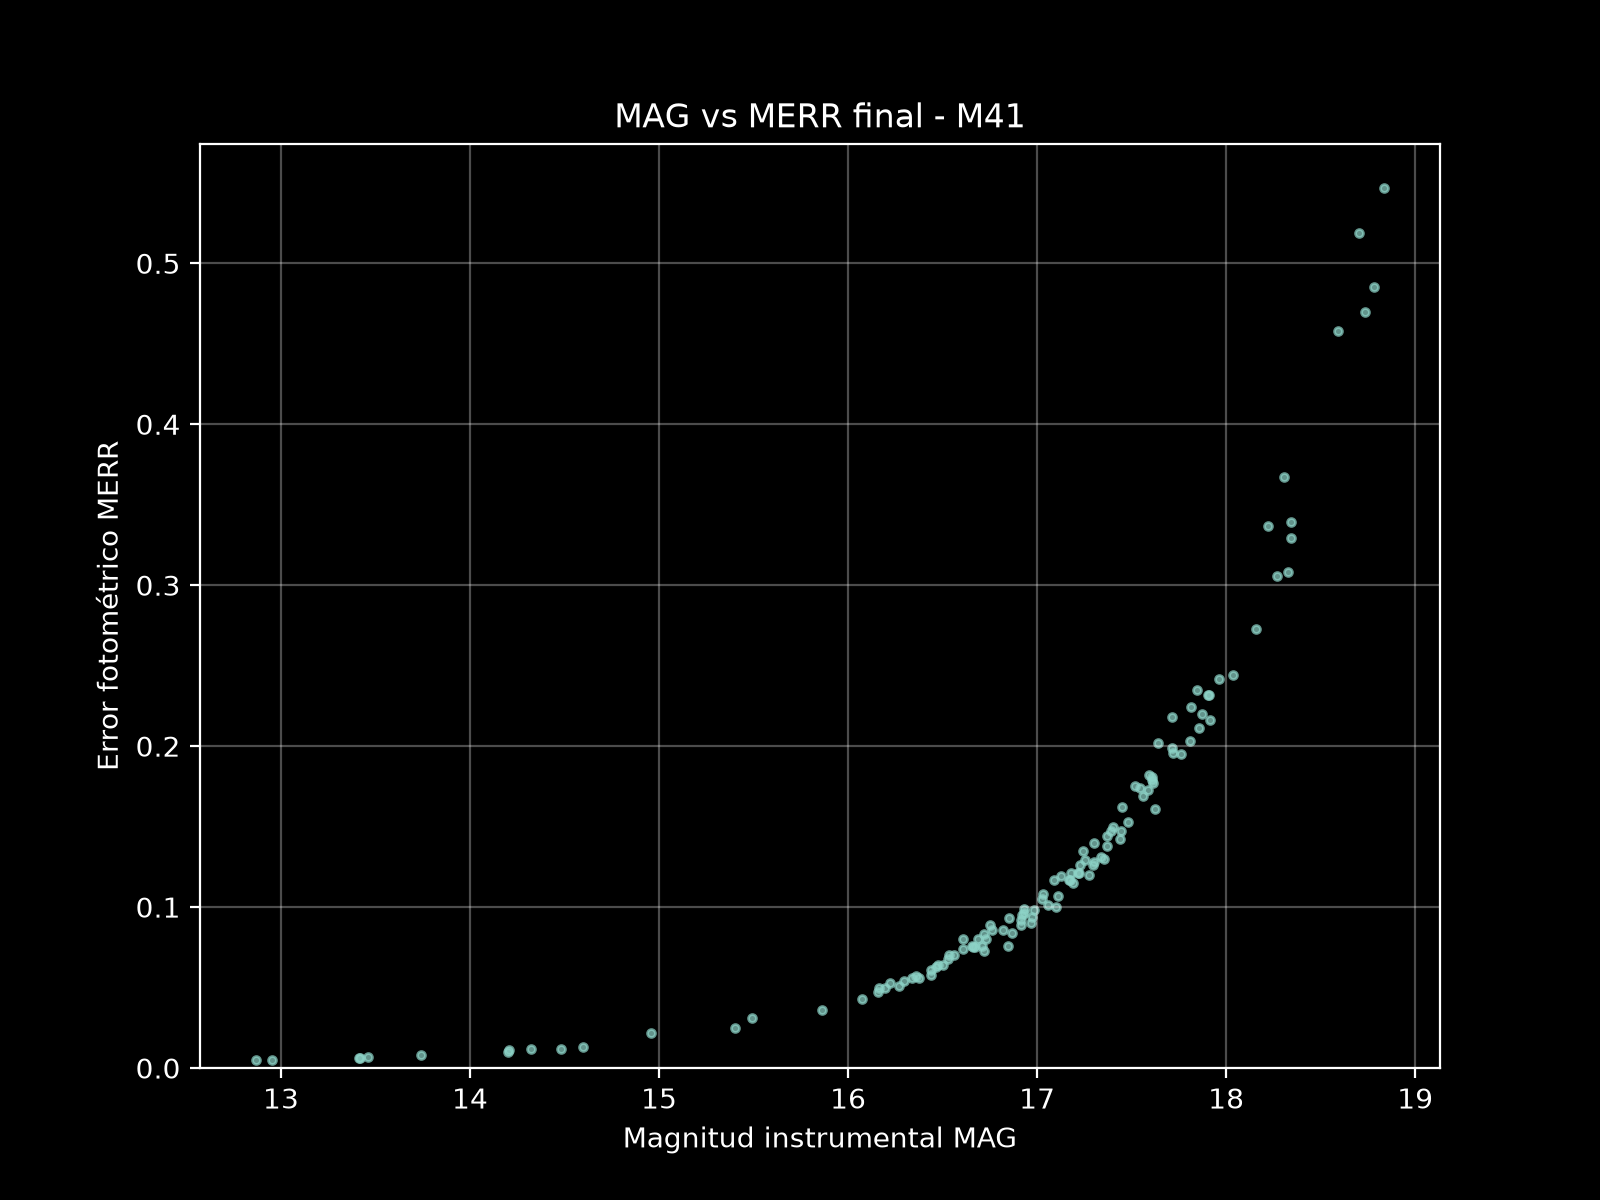
\includegraphics[width=0.65\textwidth]
{img/m91_final_mag_vs_merr.png}

\caption{
Magnitud instrumental frente a error fotométrico para M41.
}

\label{fig:m41merr}

\end{figure}


% ============================================================
% CMD INICIAL
% ============================================================

\section{Diagrama color--magnitud inicial de M92}

Utilizando las magnitudes instrumentales de \texttt{m92011.fits} y \texttt{m92015.fits} se construyó una primera versión del CMD.

El color instrumental se calculó mediante $B-V=m_B-m_V$, utilizando para cada fuente las magnitudes instrumentales obtenidas en los dos filtros.

\begin{figure}[H]

\centering

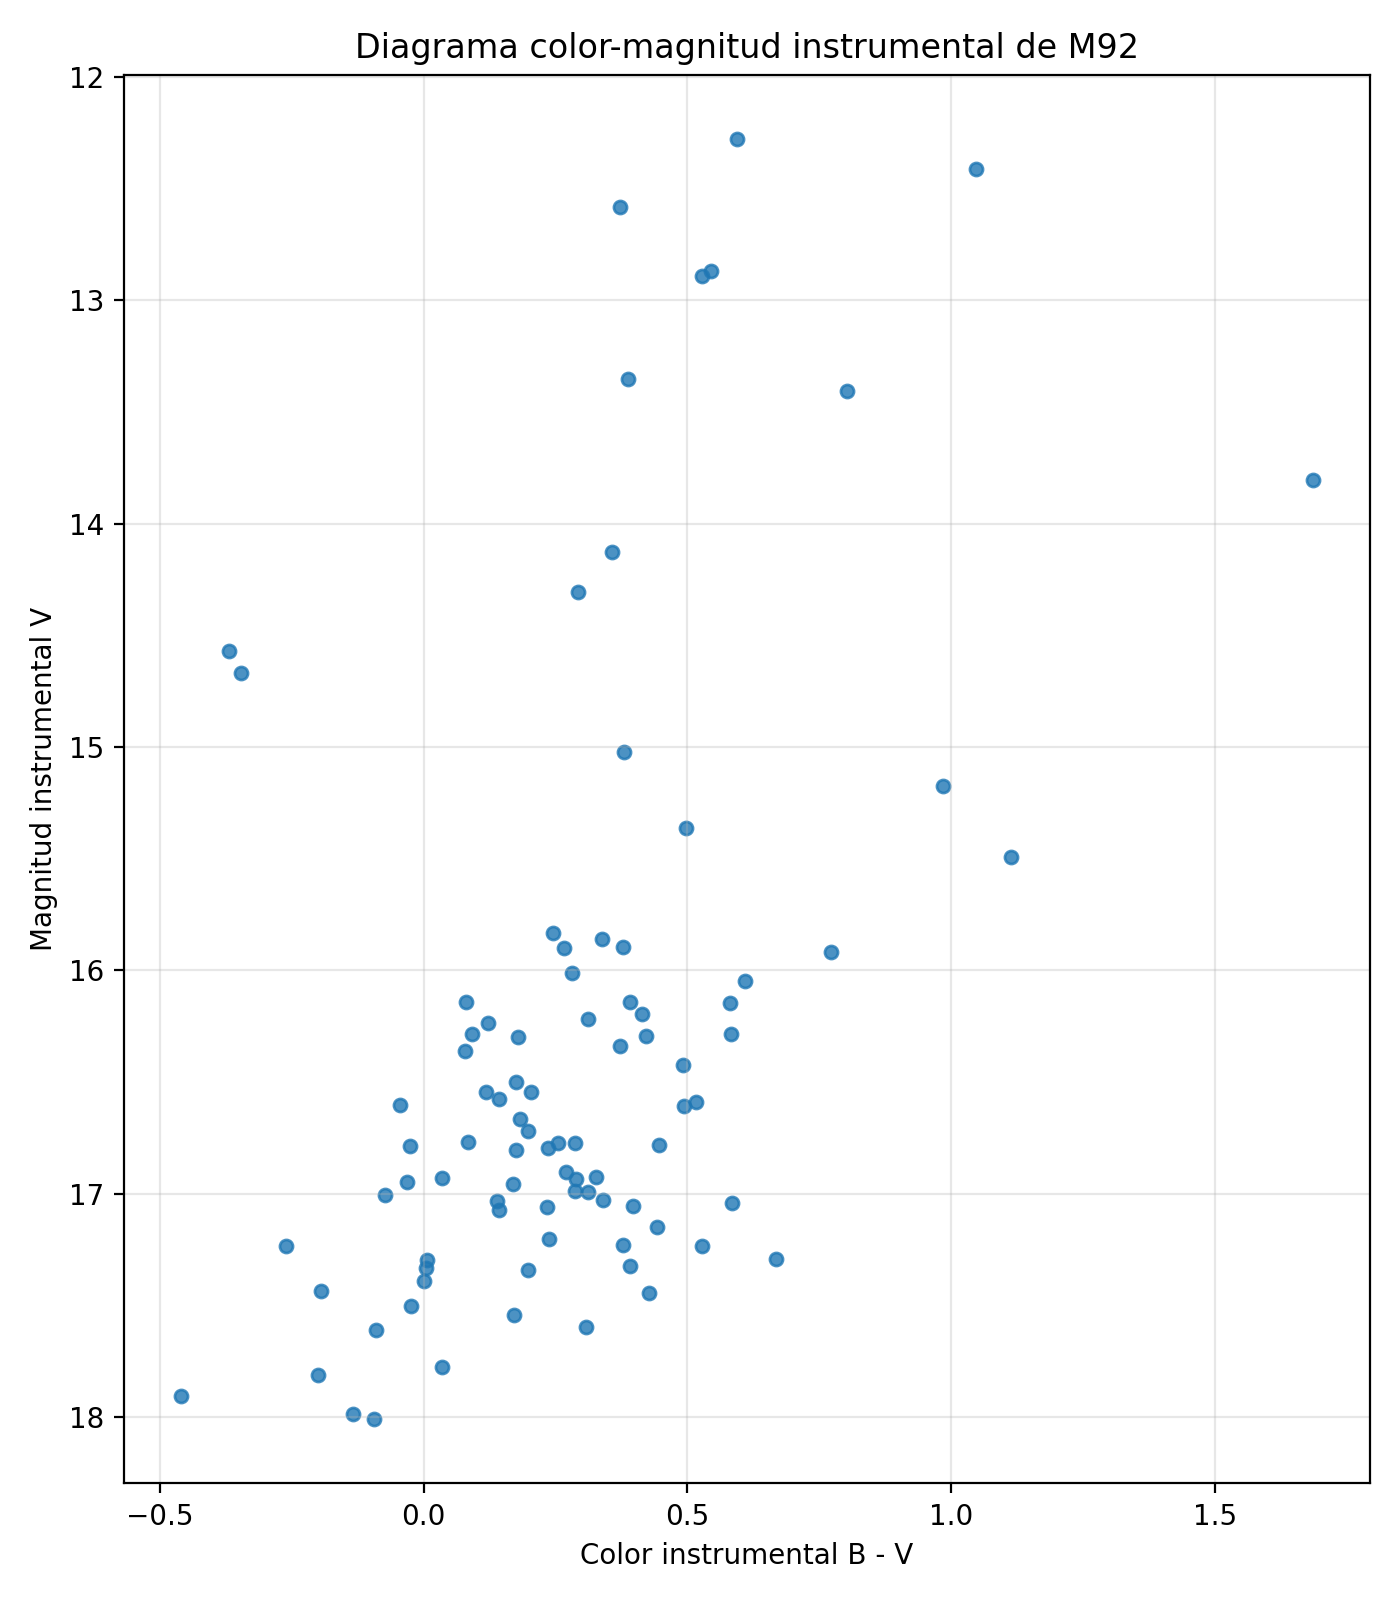
\includegraphics[width=0.65\textwidth]
{img/M92_CMD_clean.png}

\caption{
Diagrama color--magnitud instrumental inicial de M92. El eje horizontal corresponde al color $B-V$ y el eje vertical a la magnitud instrumental $V$.
}

\label{fig:cmdinicial}

\end{figure}


% ============================================================
% VECINOS RESULTADOS
% ============================================================

\section{Filtrado mediante vecinos más cercanos}

La aplicación del criterio de aislamiento permitió identificar fuentes cuya fotometría podría estar contaminada por estrellas próximas.

Para \texttt{m92011.fits}, la mediana del FWHM fue de $3.355\ {\rm pix}$ y, en consecuencia, se utilizó un radio límite de $3FWHM=10.065\ {\rm pix}$. Las estrellas con un vecino dentro de esta distancia fueron clasificadas como rechazadas y, en la muestra correspondiente a este procedimiento, se identificaron 14 fuentes que no cumplieron el criterio de aislamiento adoptado.

\begin{figure}[H]

\centering

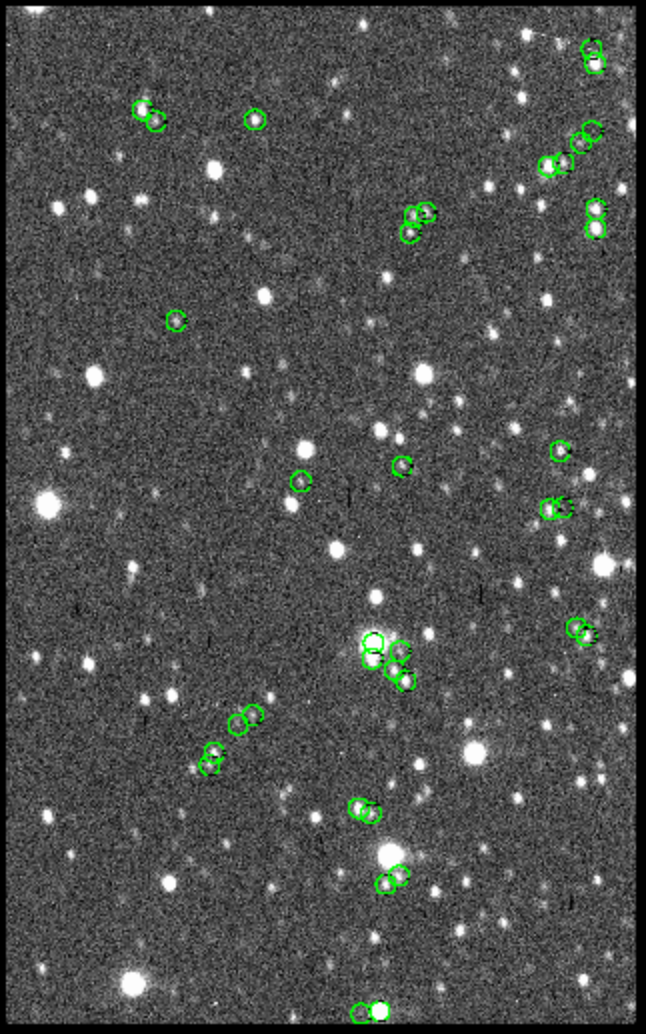
\includegraphics[width=0.65\textwidth]
{img/rechazadasVecinosCercanos.png}

\caption{
Fuentes rechazadas por presentar un vecino dentro del radio de $3\times FWHM$.
}

\label{fig:vecinosrechazados}

\end{figure}


\begin{figure}[H]

\centering

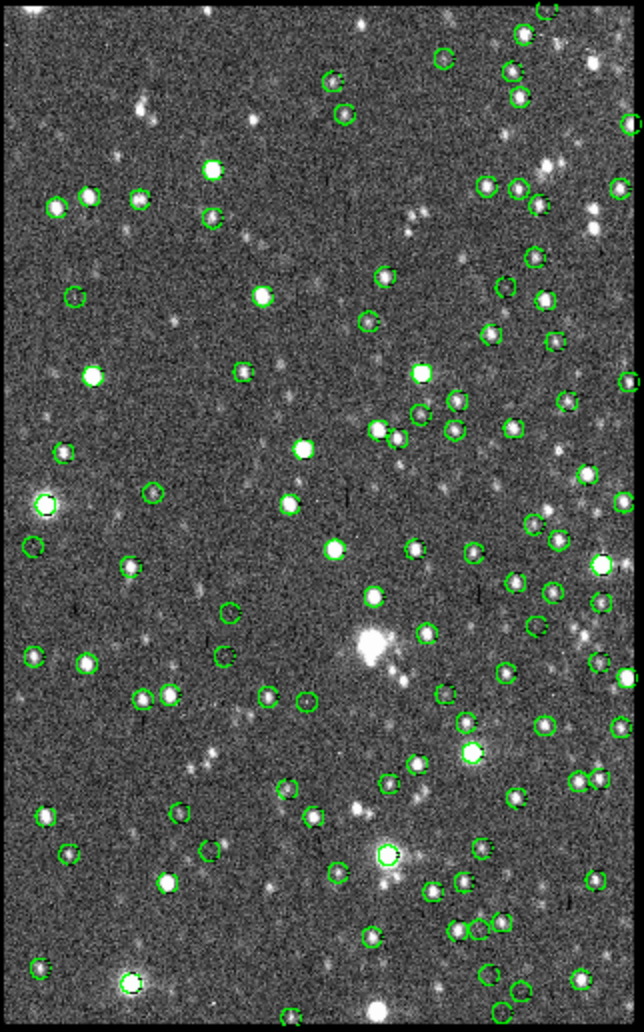
\includegraphics[width=0.65\textwidth]
{img/aceptadasVecinosCercanos.png}

\caption{
Fuentes aceptadas después de aplicar el criterio de vecinos más cercanos.
}

\label{fig:vecinosaceptados}

\end{figure}


% ============================================================
% ANILLO
% ============================================================

\section{Contaminación del anillo de cielo}

El análisis estadístico de los valores de los píxeles presentes en los anillos de cielo mostró que algunas fuentes presentaban distribuciones con una cantidad importante de valores altos.

Estos valores pueden estar asociados al flujo de estrellas vecinas dentro del anillo.


La distribución completa de los valores de los píxeles contenidos en los anillos de cielo se presenta en la Figura~\ref{fig:boxplot} del Apéndice~\ref{ap:boxplot-anillos}, donde se muestra en formato horizontal para facilitar la comparación entre las fuentes.


La fracción de valores atípicos altos permitió implementar un criterio adicional de selección.


\begin{figure}[H]

\centering

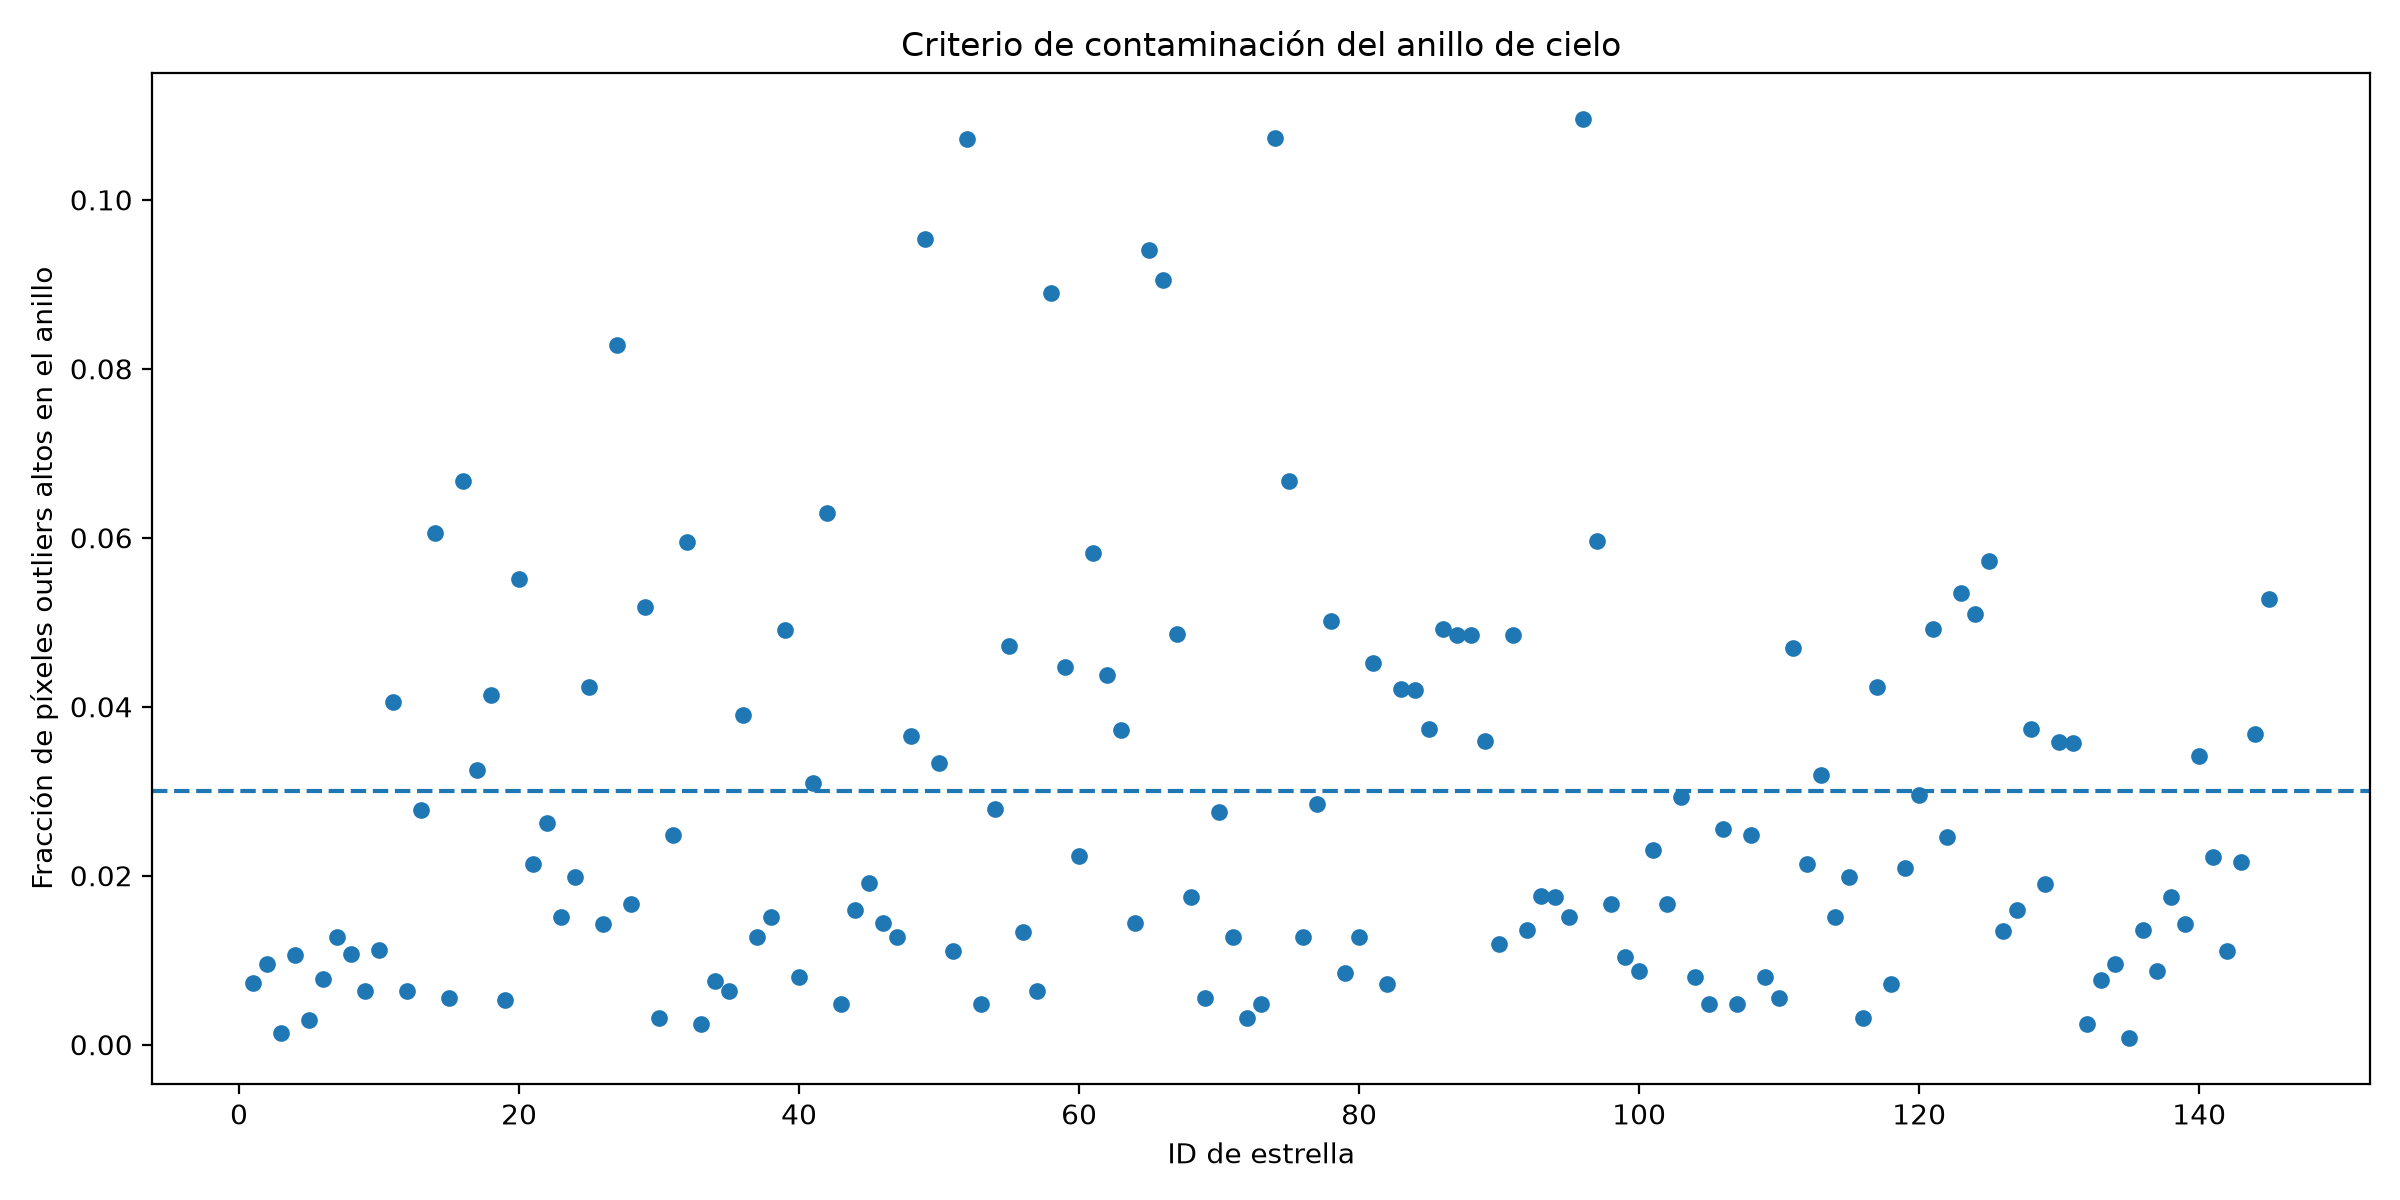
\includegraphics[width=0.80\textwidth]
{img/m92011_outliers_anillos_cielo.png}

\caption{
Fracción de píxeles atípicos altos encontrados en los anillos de cielo.
}

\label{fig:outliers}

\end{figure}


Mediante este criterio se rechazaron 28 estrellas cuyos anillos presentaron indicios de contaminación.

\begin{figure}[H]

\centering

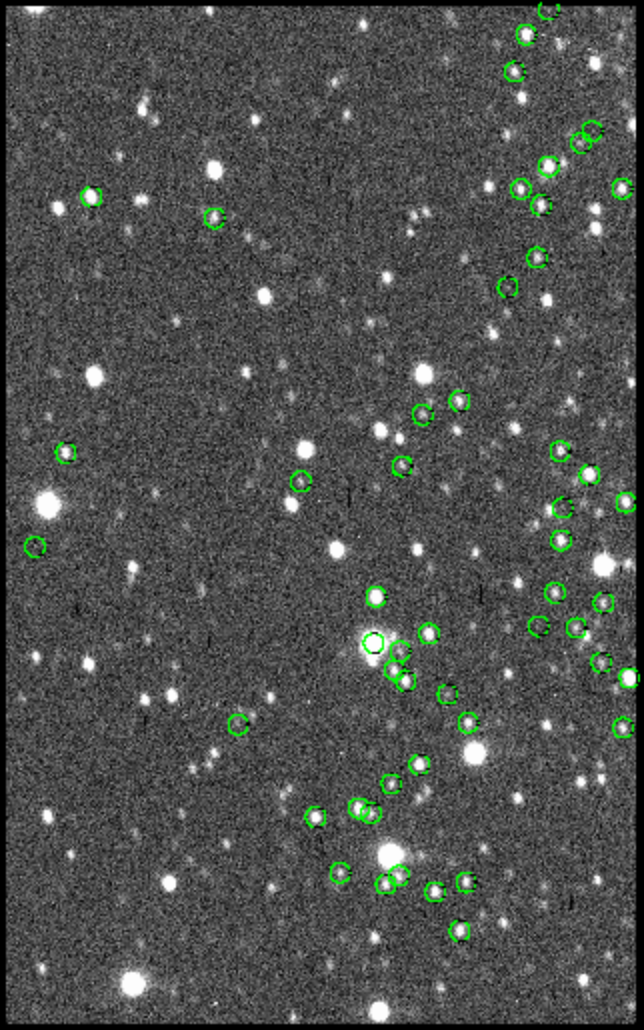
\includegraphics[width=0.65\textwidth]
{img/rechazadasAnilloCielo.png}

\caption{
Estrellas rechazadas debido a indicios de contaminación dentro del anillo utilizado para determinar el fondo local.
}

\label{fig:anillorechazadas}

\end{figure}


Las estrellas que superaron el criterio de calidad del anillo se conservaron para el análisis posterior.

\begin{figure}[H]

\centering

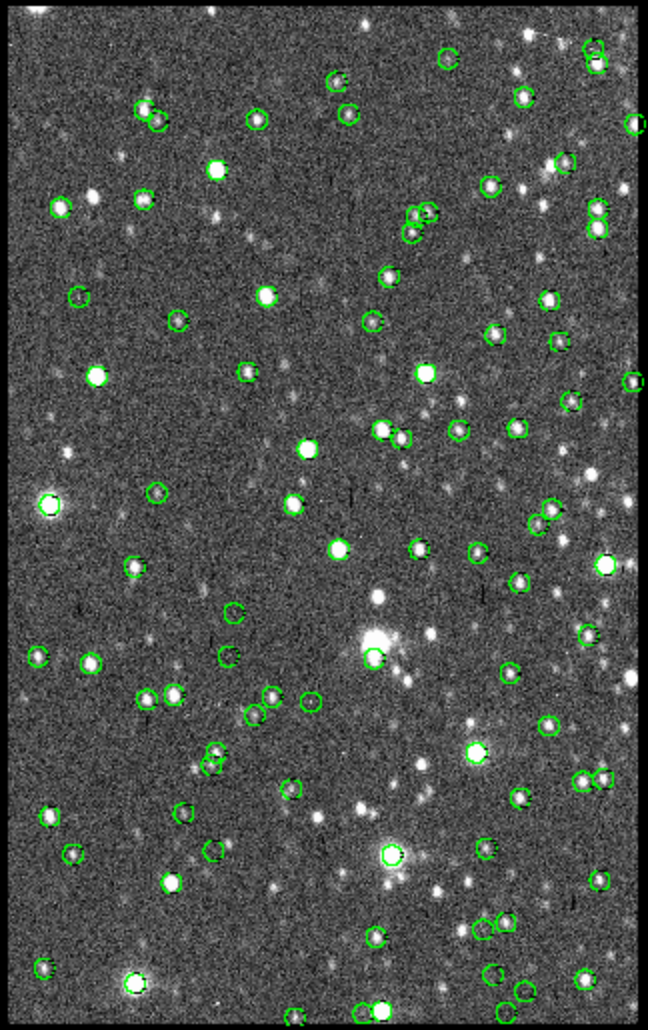
\includegraphics[width=0.65\textwidth]
{img/aceptadasAnilloCielo.png}

\caption{
Estrellas aceptadas después de aplicar el filtro de contaminación del anillo de cielo.
}

\label{fig:anilloaceptadas}

\end{figure}


% ============================================================
% CMD FINAL
% ============================================================

\section{CMD después del proceso de filtrado}

Finalmente se representaron sobre el diagrama color--magnitud las fuentes identificadas durante los diferentes procedimientos de depuración.

Esto permite visualizar qué regiones del CMD contienen estrellas rechazadas por los criterios de vecinos próximos o contaminación del fondo.


\begin{figure}[H]

\centering

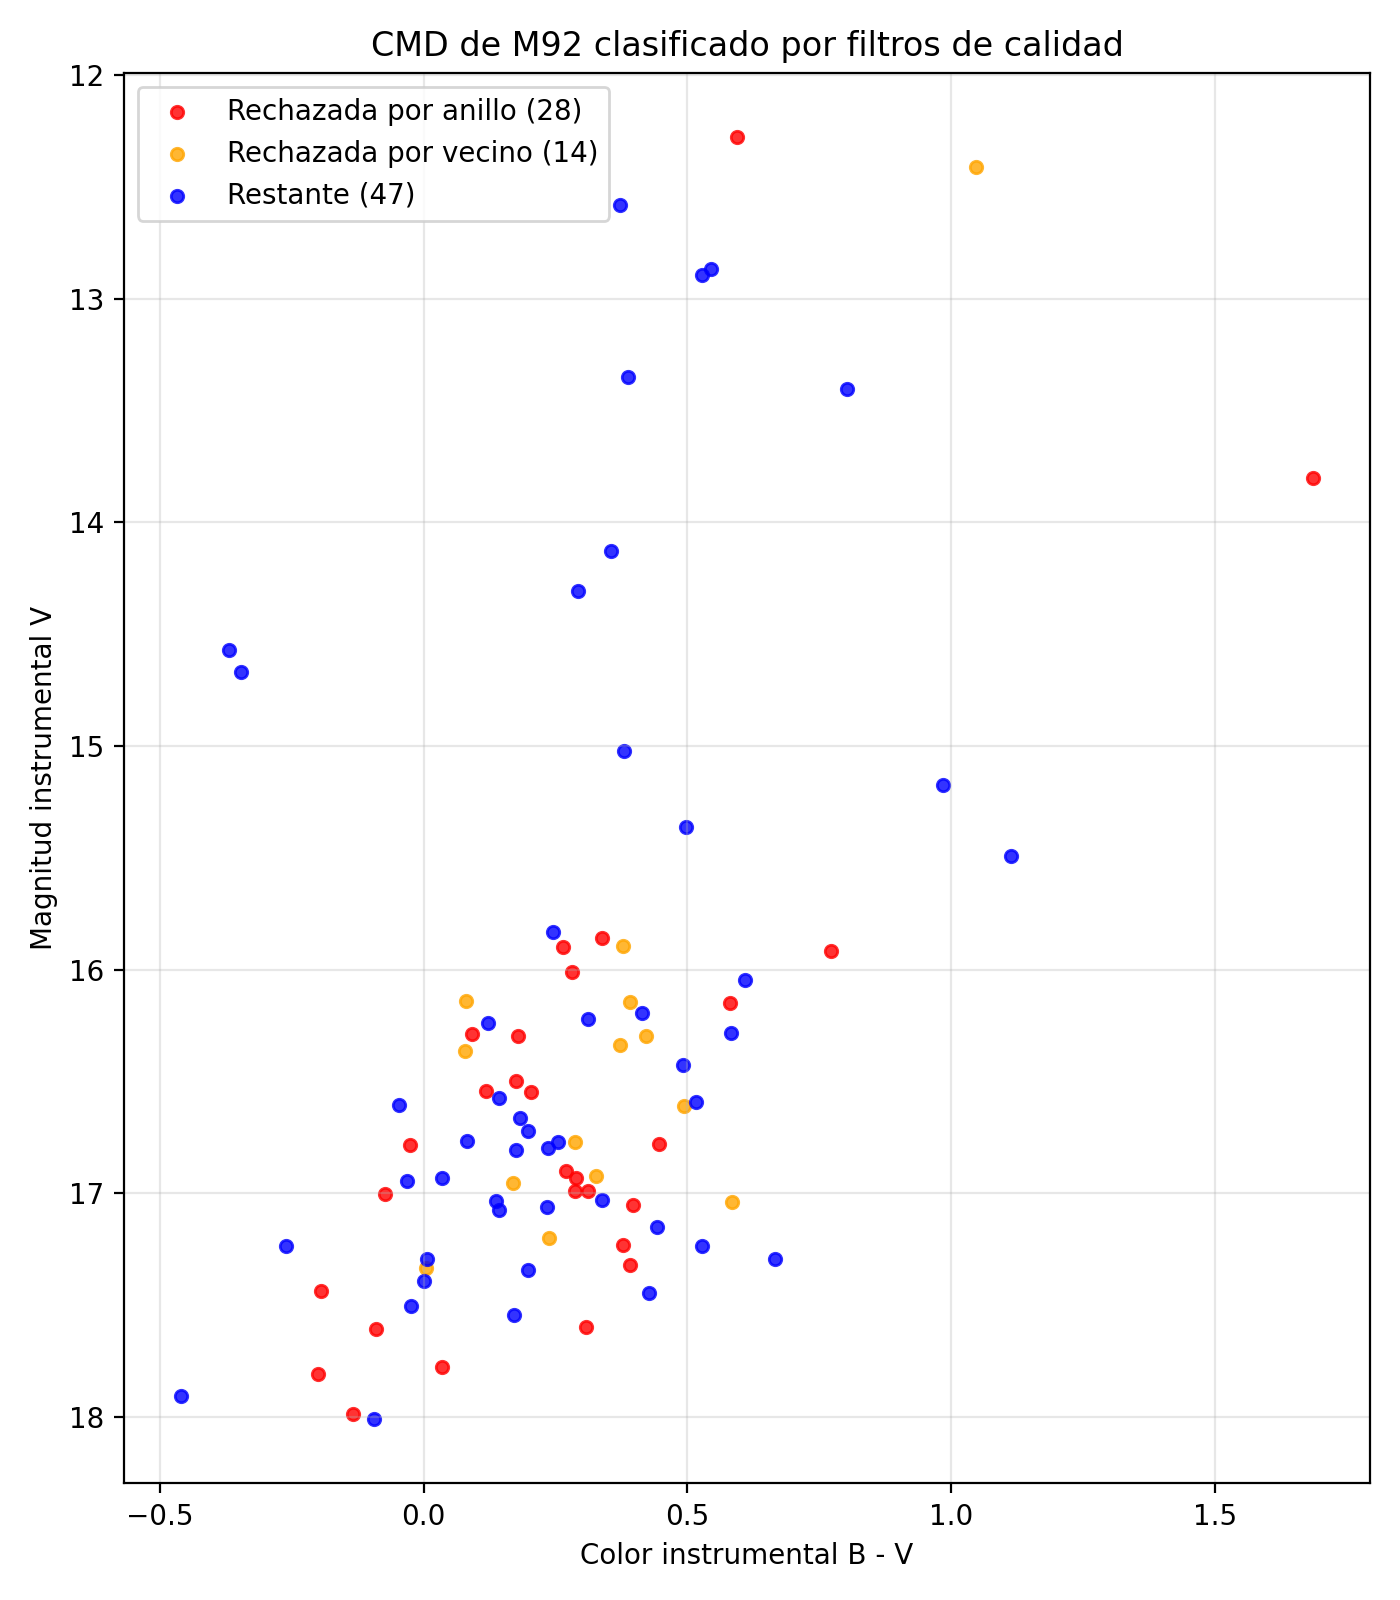
\includegraphics[width=0.68\textwidth]
{img/M92_CMD_coloreado_filtros.png}

\caption{
Diagrama color--magnitud de M92 después de aplicar los diferentes criterios de filtrado fotométrico.
}

\label{fig:cmdfinal}

\end{figure}


% ============================================================
% DISCUSIÓN GENERAL DE LOS RESULTADOS
% ============================================================

\section{Discusión general}

El procedimiento desarrollado permitió analizar diferentes etapas necesarias para transformar imágenes CCD en mediciones fotométricas instrumentales.

La reducción inicial es indispensable debido a que los valores contenidos en una imagen cruda no están producidos exclusivamente por los fotones provenientes de los objetos astronómicos. El nivel de bias, la estructura observada mediante el overscan y las variaciones de sensibilidad del detector modifican la señal registrada.

Las correcciones realizadas buscan, por tanto, que las diferencias de cuentas presentes entre diferentes estrellas representen de forma más fiel diferencias reales de flujo.

El análisis del FWHM permitió establecer una escala característica para el tamaño de las fuentes observadas. En lugar de utilizar un radio de apertura fijo e independiente de las condiciones de cada imagen, el empleo de un múltiplo del FWHM relaciona la apertura con el perfil estelar observado.

La utilización de tres veces la mediana del FWHM proporcionó un criterio uniforme para definir las aperturas utilizadas en las diferentes imágenes.

El uso de la mediana también reduce la sensibilidad a perfiles anómalos, estrellas saturadas o mediciones incorrectas individuales.

La detección automática mediante \texttt{daofind} mostró además la importancia de seleccionar adecuadamente el parámetro \texttt{threshold}.

Un umbral de detección muy pequeño incrementa la sensibilidad a fluctuaciones del fondo, mientras que uno demasiado grande elimina fuentes reales de menor señal.

El valor de 3.5 adoptado en el trabajo proporcionó un equilibrio apropiado para las imágenes estudiadas.

Las gráficas de magnitud instrumental contra error muestran la relación esperada entre intensidad y precisión fotométrica. Las estrellas brillantes poseen generalmente errores menores, mientras que el error aumenta progresivamente para objetos más débiles.

Este comportamiento es consistente con la dependencia de la incertidumbre respecto a la relación señal--ruido.

Sin embargo, una fuente puede tener una relación señal--ruido aparentemente adecuada y aun así presentar una medición sesgada si se encuentra demasiado cerca de otra estrella.

Este efecto resulta particularmente importante para un cúmulo globular como M92.

El criterio de vecinos más cercanos introducido en este trabajo proporciona una forma geométrica simple de identificar parte de estos casos.

El uso de $3\times FWHM$ como distancia mínima conecta directamente el criterio de aislamiento con la escala espacial del perfil estelar.

El segundo criterio de depuración analiza una fuente distinta de contaminación.

Incluso cuando una estrella no comparte directamente su apertura con otra fuente, una estrella cercana puede encontrarse dentro del anillo utilizado para calcular el cielo.

En estas condiciones el algoritmo puede interpretar parte de la luz estelar vecina como fondo, alterando el flujo neto calculado para la estrella principal.

La inspección de la distribución de píxeles del anillo y el análisis de valores atípicos permitió identificar casos potencialmente afectados.

La combinación de ambos criterios constituye un paso adicional respecto a una fotometría automática básica.

En lugar de utilizar directamente todas las detecciones producidas por \texttt{daofind}, se estudia la geometría local y la calidad de la región utilizada para calcular el fondo.

El CMD obtenido permite finalmente representar de forma conjunta las mediciones realizadas en los filtros $B$ y $V$.

No obstante, debe enfatizarse que las magnitudes utilizadas en esta etapa son instrumentales.

Por esta razón, la interpretación física cuantitativa del diagrama requiere un procedimiento posterior de calibración.

Para obtener magnitudes comparables con sistemas fotométricos estándar sería necesario considerar, entre otros aspectos, estrellas estándar, términos de extinción atmosférica, masa de aire, puntos cero y transformaciones de color.

Por tanto, el CMD obtenido en este trabajo debe entenderse principalmente como un diagrama instrumental que demuestra la integración de las diferentes etapas desarrolladas durante el proyecto.


% ============================================================
% CONCLUSIONES
% ============================================================

\chapter{Conclusiones}

Se implementó un flujo de trabajo para el procesamiento de imágenes astronómicas CCD utilizando IRAF, desde la reducción instrumental hasta la obtención de magnitudes mediante fotometría de apertura. La reducción de las imágenes de M92 permitió aplicar correcciones relacionadas con la región de sobrelectura, el recorte de la imagen, el nivel de polarización y el campo plano, preparando los datos para las etapas fotométricas posteriores.

La utilización de \texttt{display} e \texttt{imexamine} permitió inspeccionar las imágenes, identificar fuentes estelares y determinar propiedades fundamentales para la fotometría. En particular, la mediana del FWHM se empleó como medida representativa del tamaño de las fuentes y el radio de apertura se definió como tres veces dicho valor. Para la detección automática con \texttt{daofind} se adoptó un umbral de detección de 3.5, y las detecciones fueron revisadas posteriormente mediante \texttt{tvmark}.

La fotometría realizada mediante \texttt{phot} y \texttt{qphot} permitió obtener magnitudes instrumentales y sus errores asociados. Las gráficas de magnitud frente a error mostraron el comportamiento esperado de un aumento de la incertidumbre hacia las fuentes de menor señal. Para M92 se construyó además un diagrama color--magnitud instrumental utilizando \texttt{m92011.fits} y \texttt{m92015.fits}, asociadas a los filtros $V$ y $B$, respectivamente.

El análisis mediante vecinos más cercanos permitió identificar fuentes cuya medición podía estar afectada por estrellas localizadas dentro de una distancia de $3\times FWHM$. De forma complementaria, el estudio estadístico de los anillos de cielo permitió reconocer casos en los que la estimación del fondo local podía estar contaminada por estrellas próximas. La combinación de ambos criterios proporcionó una muestra fotométrica más depurada para la construcción del diagrama color--magnitud final.

En conjunto, el procedimiento desarrollado constituye una base para extender el trabajo hacia una calibración fotométrica completa y una interpretación física más profunda del diagrama color--magnitud de M92.


% ============================================================
% TRABAJO FUTURO
% ============================================================

\section{Trabajo futuro}

Una continuación natural de este trabajo consiste en realizar la calibración de las magnitudes instrumentales obtenidas.

Para ello será necesario determinar el punto cero fotométrico y estudiar las correcciones relacionadas con la extinción atmosférica y la masa de aire.

También puede ser necesario considerar términos de color que permitan transformar las magnitudes instrumentales al sistema fotométrico estándar.

Una vez obtenidas magnitudes calibradas, el CMD de M92 podría compararse con datos publicados y con modelos de evolución estelar.

Esto permitiría estudiar características como la secuencia principal, el punto de giro, la rama de gigantes y otras regiones evolutivas del cúmulo.

Otra extensión importante corresponde a la utilización de fotometría de PSF.

La fotometría de apertura funciona adecuadamente para estrellas suficientemente aisladas, pero pierde precisión cuando existe un alto grado de superposición entre perfiles estelares.

La fotometría de PSF modela simultáneamente la distribución espacial de las fuentes y podría permitir conservar estrellas que actualmente deben eliminarse mediante el criterio de vecinos cercanos.

Finalmente, una comparación sistemática entre fotometría de apertura y fotometría de PSF permitiría cuantificar el efecto de la densidad estelar sobre la precisión de las magnitudes obtenidas.


% ============================================================
% BIBLIOGRAFÍA
% ============================================================

% Solo se incluyen en la bibliografía las referencias citadas explícitamente en el texto.

\bibliographystyle{aa_url}
\bibliography{global}


% ============================================================
% APÉNDICES
% ============================================================

\appendix

\appendixpage

\noappendicestocpagenum

\addappheadtotoc


% ============================================================
% APÉNDICE A
% ============================================================

\chapter{Comandos principales utilizados en IRAF}

\section{Reducción}

Para realizar la reducción CCD se cargaron primero los paquetes \texttt{noao}, \texttt{imred} y \texttt{ccdred}. La inspección detallada del encabezado de una imagen se efectuó, por ejemplo, con \texttt{imhead m92011.fits long+}. Posteriormente se accedió a la configuración de \texttt{ccdproc} mediante \texttt{epar ccdproc} y, una vez establecidos los parámetros correspondientes, la reducción se ejecutó sobre la imagen con \texttt{ccdproc m92011.fits}.


% ------------------------------------------------------------

\section{Inspección de estrellas}

La inspección interactiva de las fuentes se realizó cargando primero la imagen \texttt{m92011.fits} en el marco gráfico mediante \texttt{display m92011.fits 1} y ejecutando después \texttt{imexamine m92011.fits}. Esta combinación permitió seleccionar estrellas directamente sobre la imagen y revisar sus perfiles, posiciones y propiedades asociadas.


% ------------------------------------------------------------

\section{Detección automática}

Para la detección automática en \texttt{m92011.fits} se utilizó \texttt{daofind}, indicando como archivo de salida \texttt{m92011.coo}, un \texttt{fwhmpsf} de 3.355 píxeles, el valor de \texttt{sigma} obtenido para el fondo y un \texttt{threshold} de 3.5. La opción \texttt{verify-} se empleó para ejecutar la tarea sin solicitar confirmación interactiva para cada detección.


% ------------------------------------------------------------

\section{Marcado de coordenadas}

Para comprobar visualmente las coordenadas detectadas se volvió a cargar \texttt{m92011.fits} con \texttt{display} y se utilizó \texttt{tvmark} sobre el marco 1, tomando las posiciones desde \texttt{m92011.coo}. Las fuentes se representaron mediante círculos de radio 5 píxeles y un color de marcado definido por IRAF; la numeración de las fuentes puede activarse o desactivarse con las opciones \texttt{number+} y \texttt{number-}, respectivamente.


% ------------------------------------------------------------

\section{Fotometría}

La fotometría de apertura de \texttt{m92011.fits} se realizó con \texttt{phot}, utilizando \texttt{m92011.coo} como archivo de coordenadas y \texttt{m92011.mag} como archivo de salida. Las opciones \texttt{interac-} y \texttt{verify-} permitieron aplicar los parámetros previamente establecidos de forma automática a todas las fuentes incluidas en la lista.


% ------------------------------------------------------------

\section{Extracción de resultados}

Finalmente, los resultados almacenados en \texttt{m92011.mag} se extrajeron mediante \texttt{txdump}. Se seleccionaron los campos \texttt{XCENTER}, \texttt{YCENTER}, \texttt{MAG} y \texttt{MERR}, y la salida se redirigió al archivo \texttt{m92011\_final.dat}. Este archivo concentró las coordenadas, magnitudes instrumentales y errores utilizados en los análisis posteriores.


% ============================================================
% FIGURA COMPLEMENTARIA: ANILLOS DE CIELO
% ============================================================

\chapter{Distribución de los anillos de cielo}
\label{ap:boxplot-anillos}

La Figura~\ref{fig:boxplot} reúne la distribución de los valores de los píxeles contenidos dentro de los anillos de cielo de las estrellas analizadas en \texttt{m92011.fits}. Debido a la cantidad de fuentes representadas, la gráfica se presenta en una página horizontal para conservar la legibilidad de las etiquetas y facilitar la comparación entre las distribuciones.

\clearpage
\begin{landscape}
\begin{figure}[p]
\centering
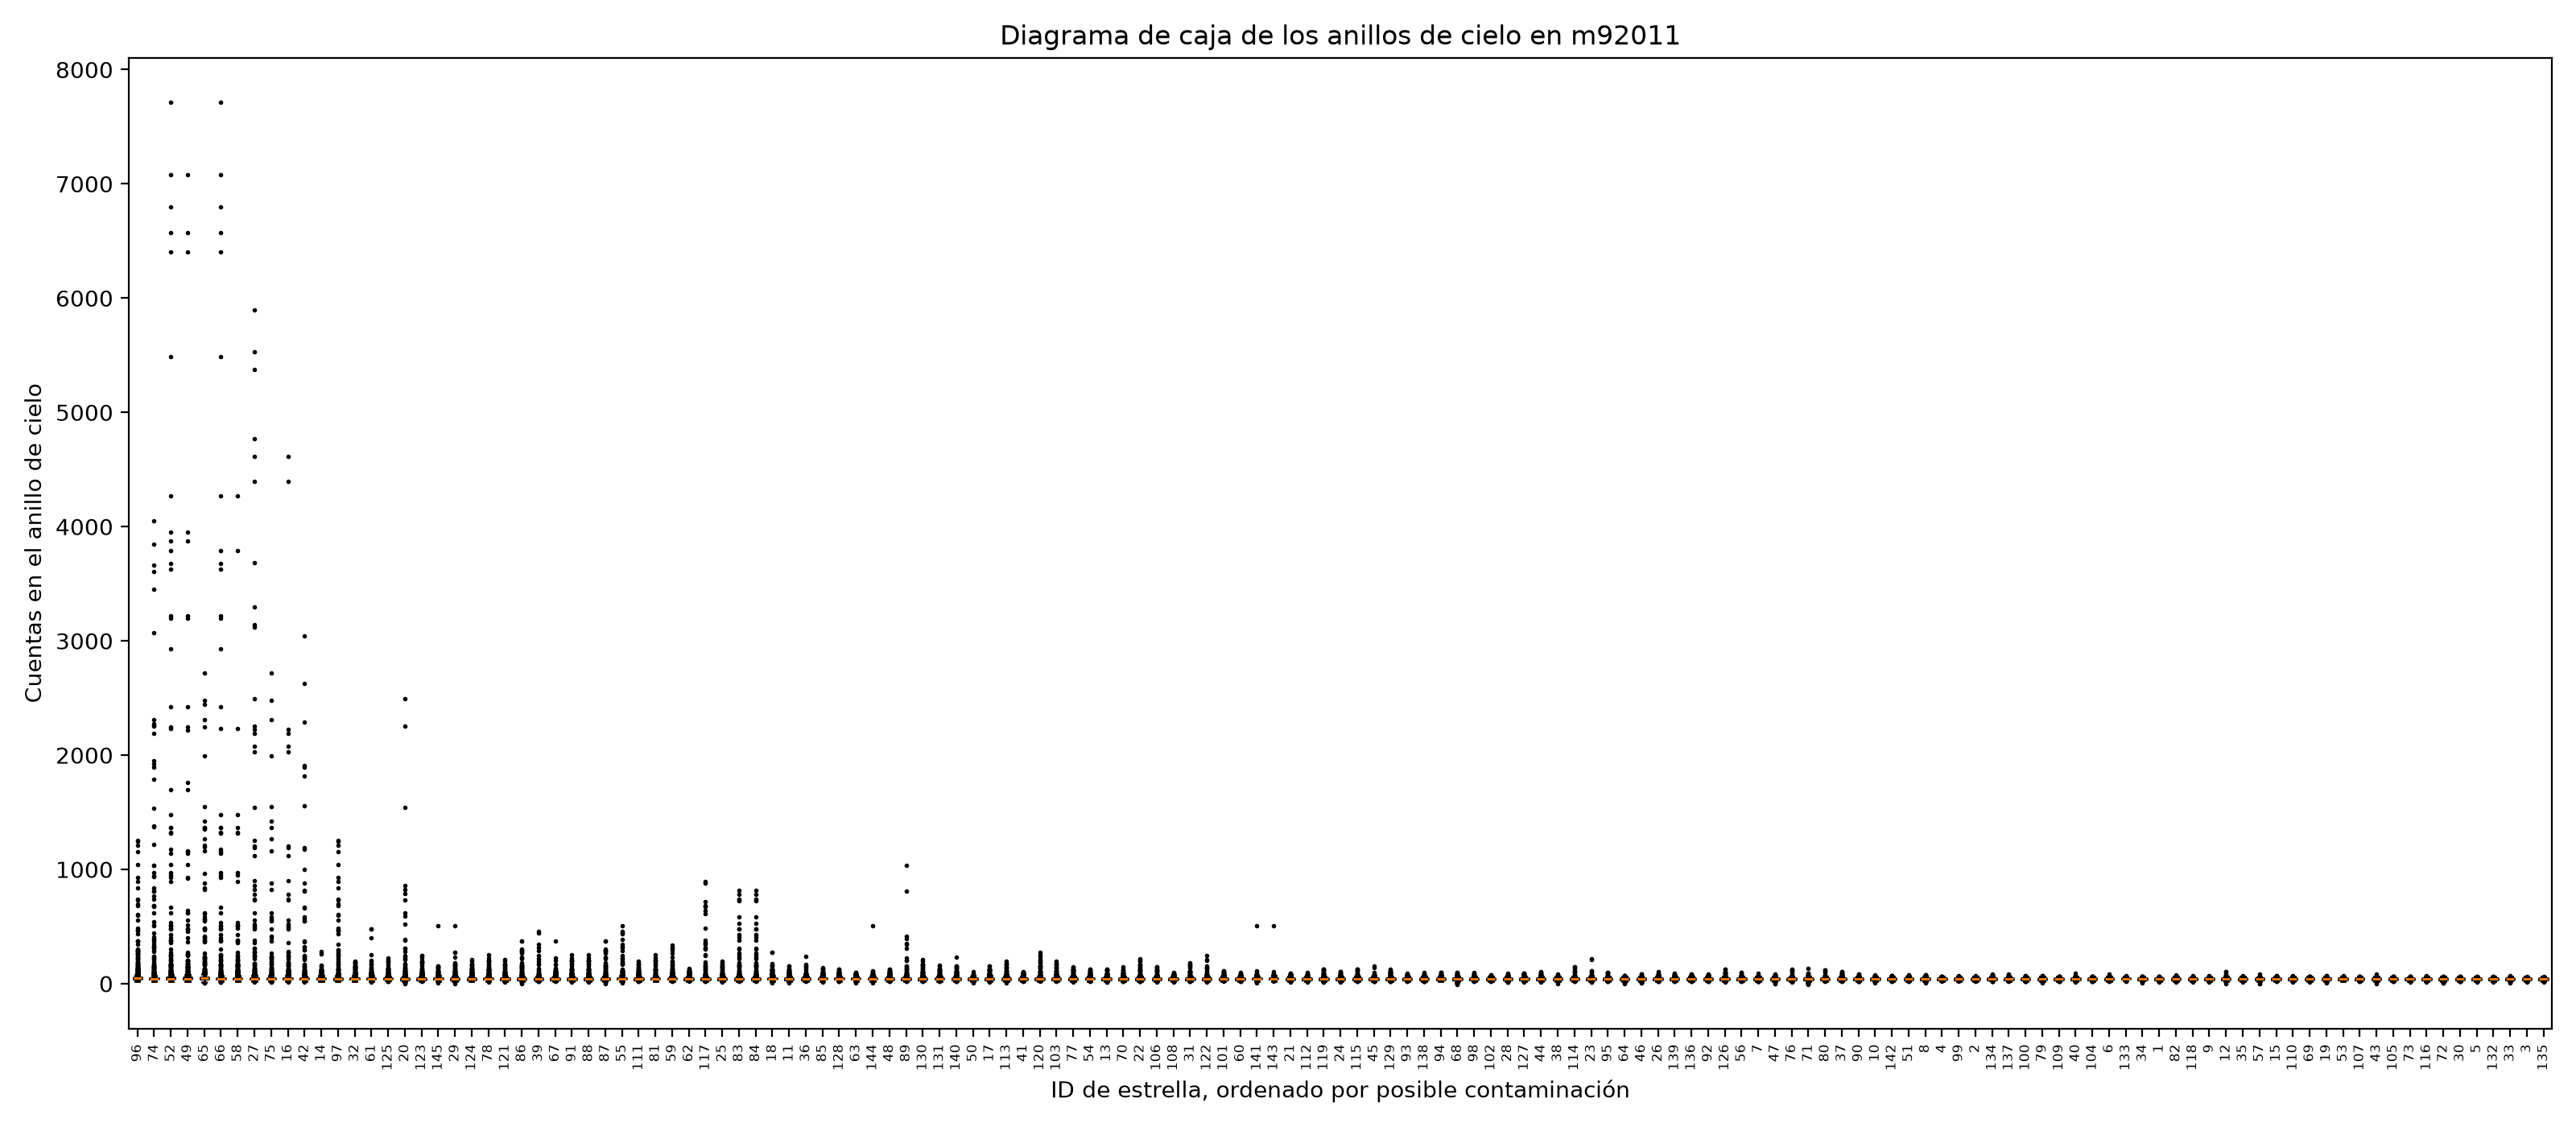
\includegraphics[width=0.96\linewidth,height=0.82\textheight,keepaspectratio]
{img/m92011_boxplot_anillos_cielo.png}
\caption{Distribución de los valores de los píxeles contenidos dentro de los anillos de cielo de las estrellas de \texttt{m92011.fits}. La figura se presenta en orientación horizontal para permitir la visualización completa de las fuentes analizadas.}
\label{fig:boxplot}
\end{figure}
\end{landscape}
\clearpage

% ============================================================
% MATERIAL COMPLEMENTARIO
% ============================================================

\chapter{Material complementario}

Los códigos utilizados para procesamiento estadístico, análisis de vecinos más cercanos, inspección de los anillos de cielo y construcción del CMD se conservaron como material complementario del proyecto.

Los repositorios asociados al trabajo son \url{https://github.com/sserranop1/LAB.5} y \url{https://github.com/sserranop1/M41}.


% ============================================================
% FIN
% ============================================================

\end{document}
